\chapter{Bavaria ancient DNA}
\label{chapterlabel4}

\section{Introduction}

Throughout the Pleistocene and Holocene, Germany has been the setting for many population movements and admixture events of modern humans. The Swabian Alps is home to some of the earliest pieces of symbolic art, dated to at least 32kya \cite{conard2009female} and musical instruments dated to 40kya \cite{conard2009new}, both assigned to the Aurignacian tradition. 

Later, the region was also home to one of the first Neolithic traditions in the \textit{Linearbandkeramik} (LBK), a key culture in the Neolithisation of Europe. Early LBK populations across Germany mixed with the preceding Mesolithic hunter gatherer populations \cite{Lipson2017b, mathieson2015genome, Haak2015,gunther2015ancient, Hofmanova2016}. At the end of the Neolithic, a new ancestry was detected \cite{Haak2015, Allentoft2015}  in concert with the arrival of the Corded Ware Complex \cite{furholt2003absolutchronologische}, most closely related to the Yamnaya Pastoralists from the Pontic-Capsian Steppe. Recent studies using ancient DNA have shown that the arrival of Steppe-related ancestry in Europe occurred no earlier than 2700BC \cite{furtwangler2020ancient} and spread widely shortly after.

During the Bronze Age, cultures closely related to Yamnaya, such as Bell Beakers, Corded Ware and Unetice \cite{Haak2015} appeared across Germany at sites such as Kromsdorf \cite{lee2012emerging} and Tollense \cite{jantzen2011bronze, brinker2013human}. It was later dominated by Iron Age cultures such as Hallstatt and La Tène, which have been shown to be partially continuous with the preceding Bell Beaker culture \cite{Brunel12791}. 
 
In the present-day, Germany represents a boundary point between East and West Europe, with a relatively sharp genetic boundary occurring between Germany and Poland to the east, given their close geographic proximity \cite{novembre2008genes, kayser2005significant, veeramah2011genetic}. However, within Germany, SNP-based studies have shown that there is only very weak substructure \cite{steffens2006snp}. Questions remain as to the origin of this East-West structure; is it recent structure, or did it exist during the Middle Ages or earlier? 

Cherry-Tree cave, or \textit{Kirschbaumhöhle}, represents a unique opportunity to study a transect of southern German samples from the Neolithic to the present-day. The cave represents a relatively untouched layer of stratigraphy, with a large series of radiocarbon dates revealing that human and animal inhabitation of the cave stretches back until at least the Michelsberg Culture in the Early Neolithic \cite{botigue2017ancient}. 

Here, I analyse novel data from 11 medium-to-high coverage samples from two sites from Southern Germany and one site from from Southern Austria. In particular, the samples from Kirschbaumhöhle span from the Late Neolithic to the Iron Age, providing an opportunity to study a time transect in a narrow geographic region (Table. \ref{tab:BavariaSampleInfo}). 

A collaborator, Prof. Joachim Burger, Johannes Gutenberg University Mainz, posed the following three questions. 

\begin{enumerate}
\item \textbf{Second Neolithic immigration wave}. One of the samples (Erg1) is thought to have belonged to the first wave of farmers carrying farming technology from the near-east to Europe, and another (DIN2) to the second wave. Do we observe genetic differences between the two waves of samples and do they show evidence of previously reported hunter-gatherer admixture?
\item \textbf{Cherry Tree Cave}. Do we see evidence of genetic continuity from from the Late Neolithic through to the Iron Age in Cherry Tree Cave?
\item \textbf{Germanic / Slavic divide}. Is there a distinction between the Germanic and Slavic samples from the Middle Age samples? How do these populations compare to the preceding samples from the Bronze and Iron ages?
\end{enumerate}

\section{Methods}

\subsection{Data generation}

Eleven whole-genomes of ancient individuals were generated by collaborators at the Johannes Gutenberg, University of Mainz, Germany. The estimated radiocarbon dates range from 5200B to 1060AD (Fig. \ref{fig:chapter4_intro_SamplesDates}). Six of the samples were found in Cherry-Tree Cave in the Bavarian district of Forchheim, four from futher South in the region of Dingolfing/Essenbach and one sample from Molzbichl in southern Austria (Fig. \ref{fig:chapter4_intro_SamplesMap}). The samples had a median coverage of 4.84x and ranged from 0.7x to 17.52x. Full details of coverage, location and dates are given in Table \ref{tab:BavariaSampleInfo}.

I was given the data of each newly sequenced sample in \texttt{vcf} format. 

\begin{figure}[htp]
    \centering
    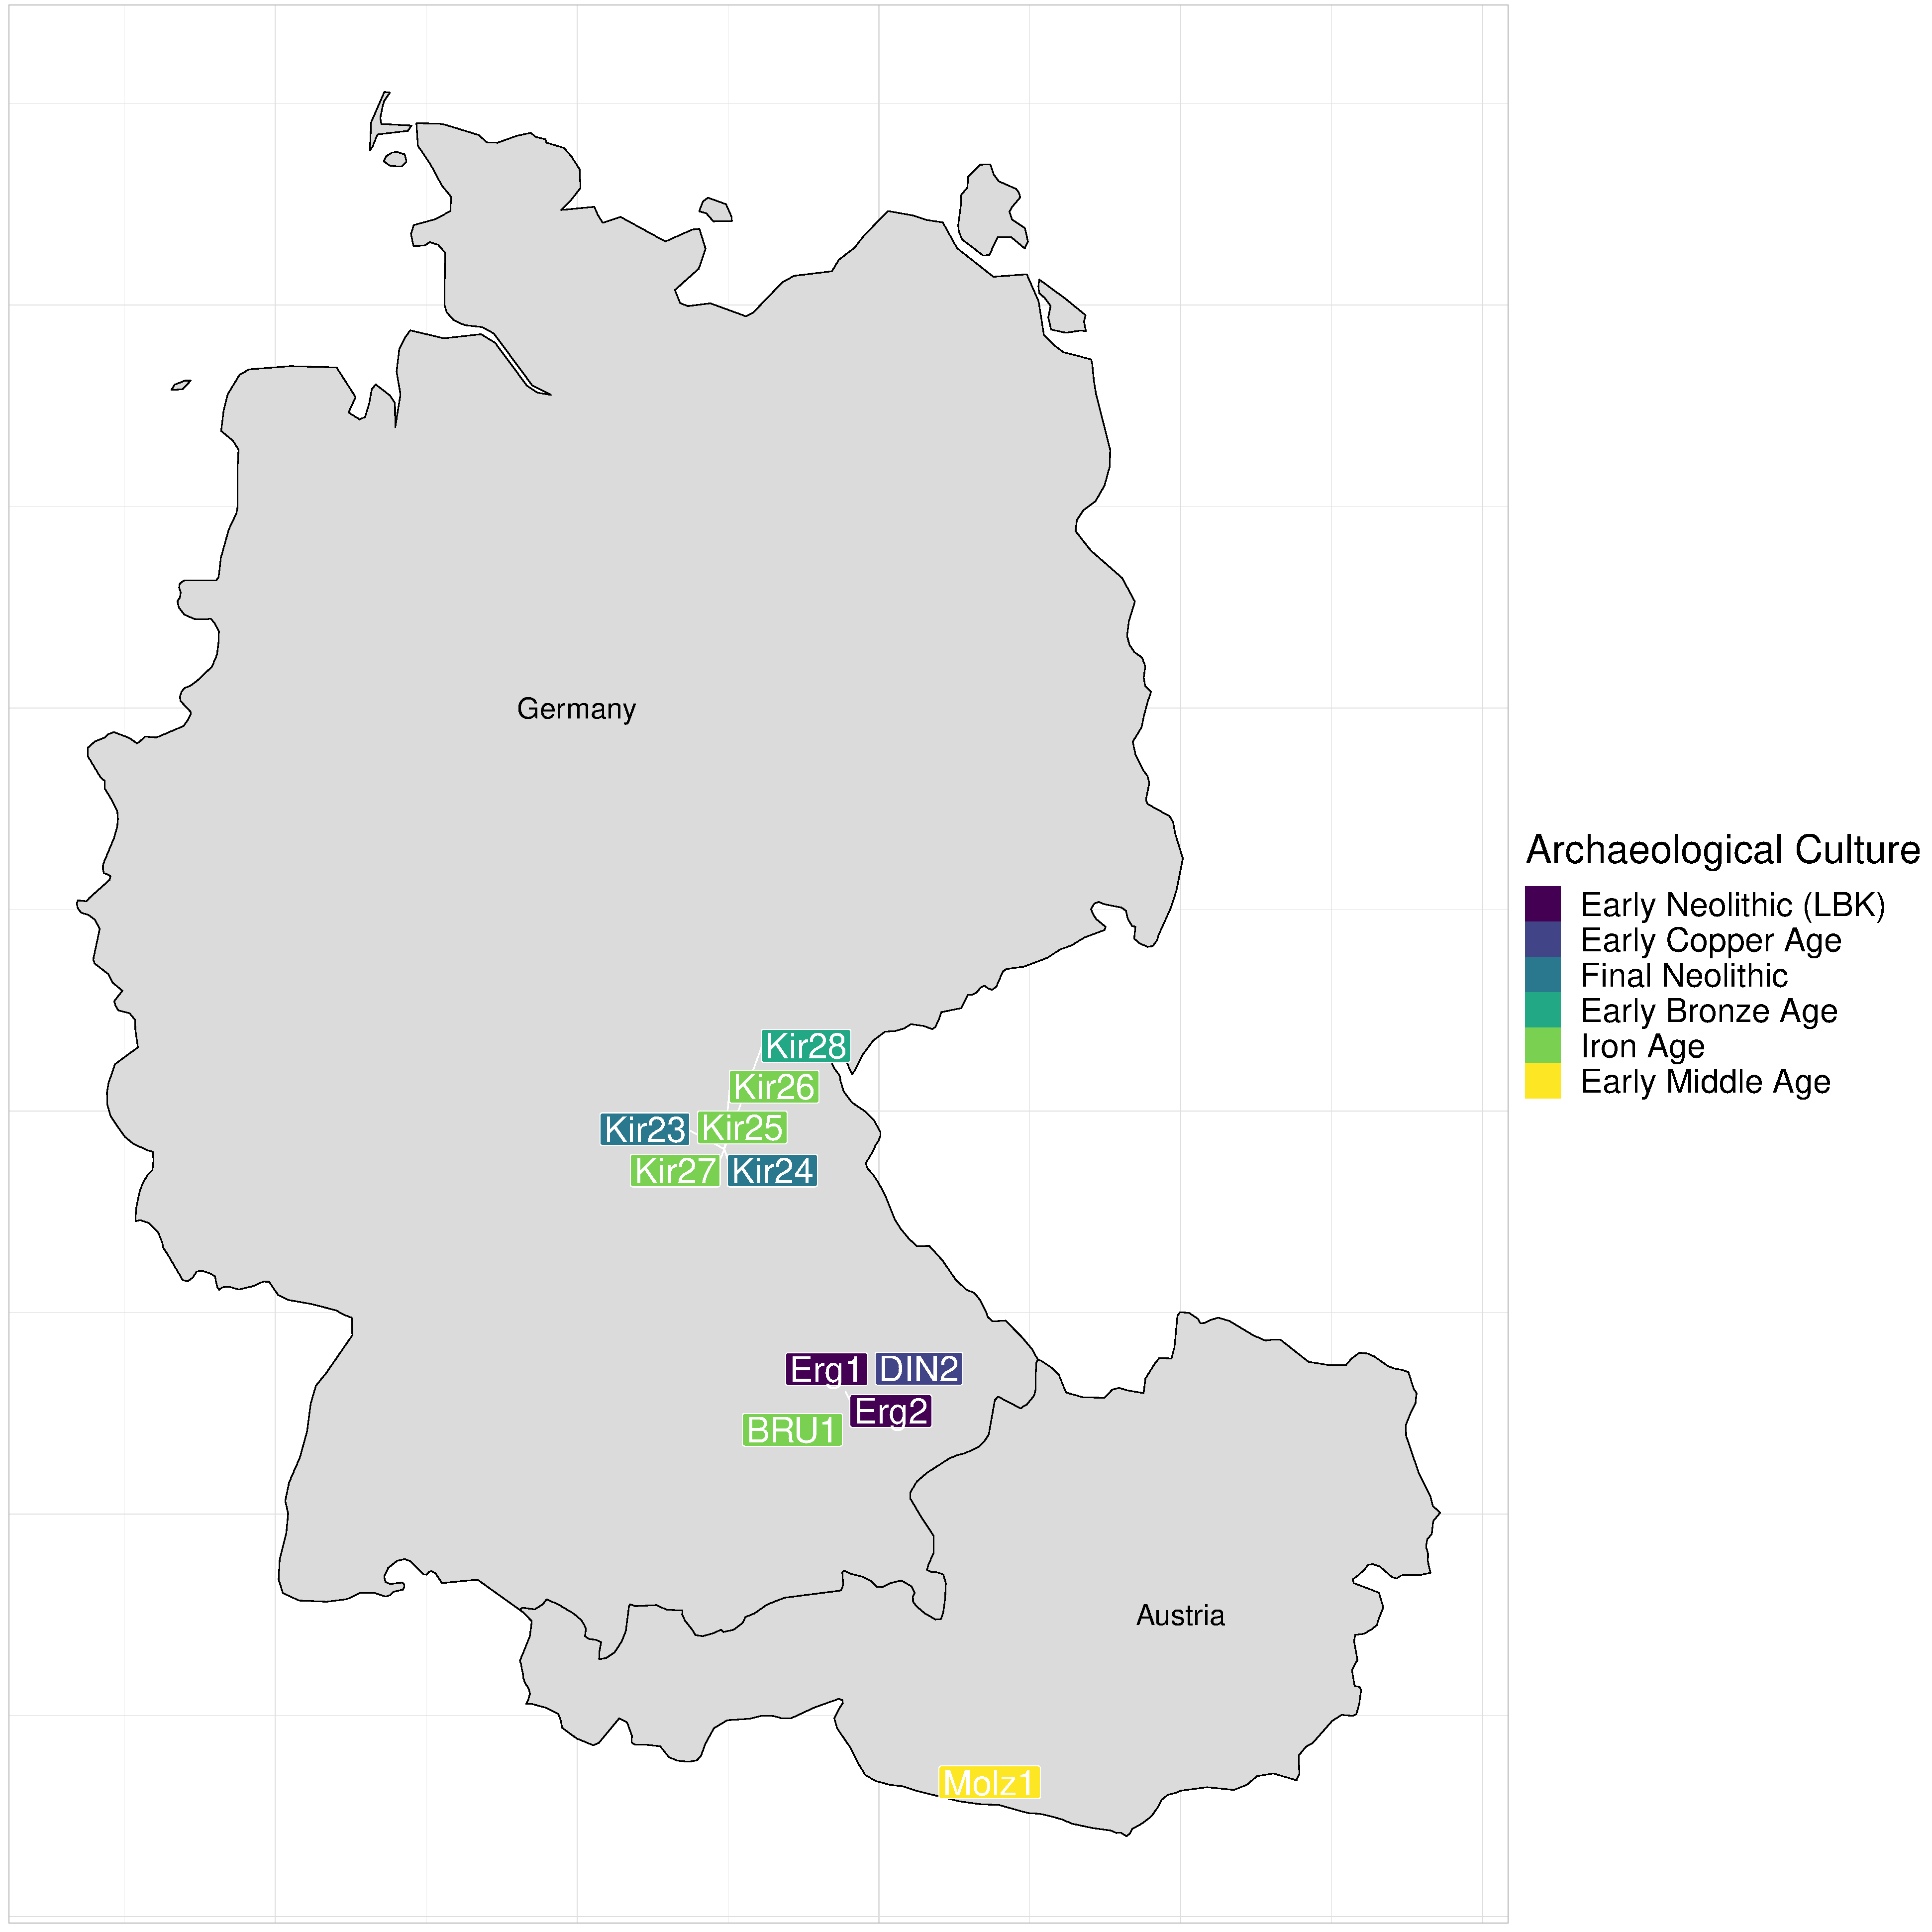
\includegraphics[width=1.0\textwidth]{../images/chapter4/sample_map.pdf}
    \caption{Map of newly sequenced ancient individuals, positioned according to where they were excavated. Colour on label corresponds to archaeological culture which they were found. }
    \label{fig:chapter4_intro_SamplesMap}
\end{figure}

\begin{figure}[htp]
    \centering
    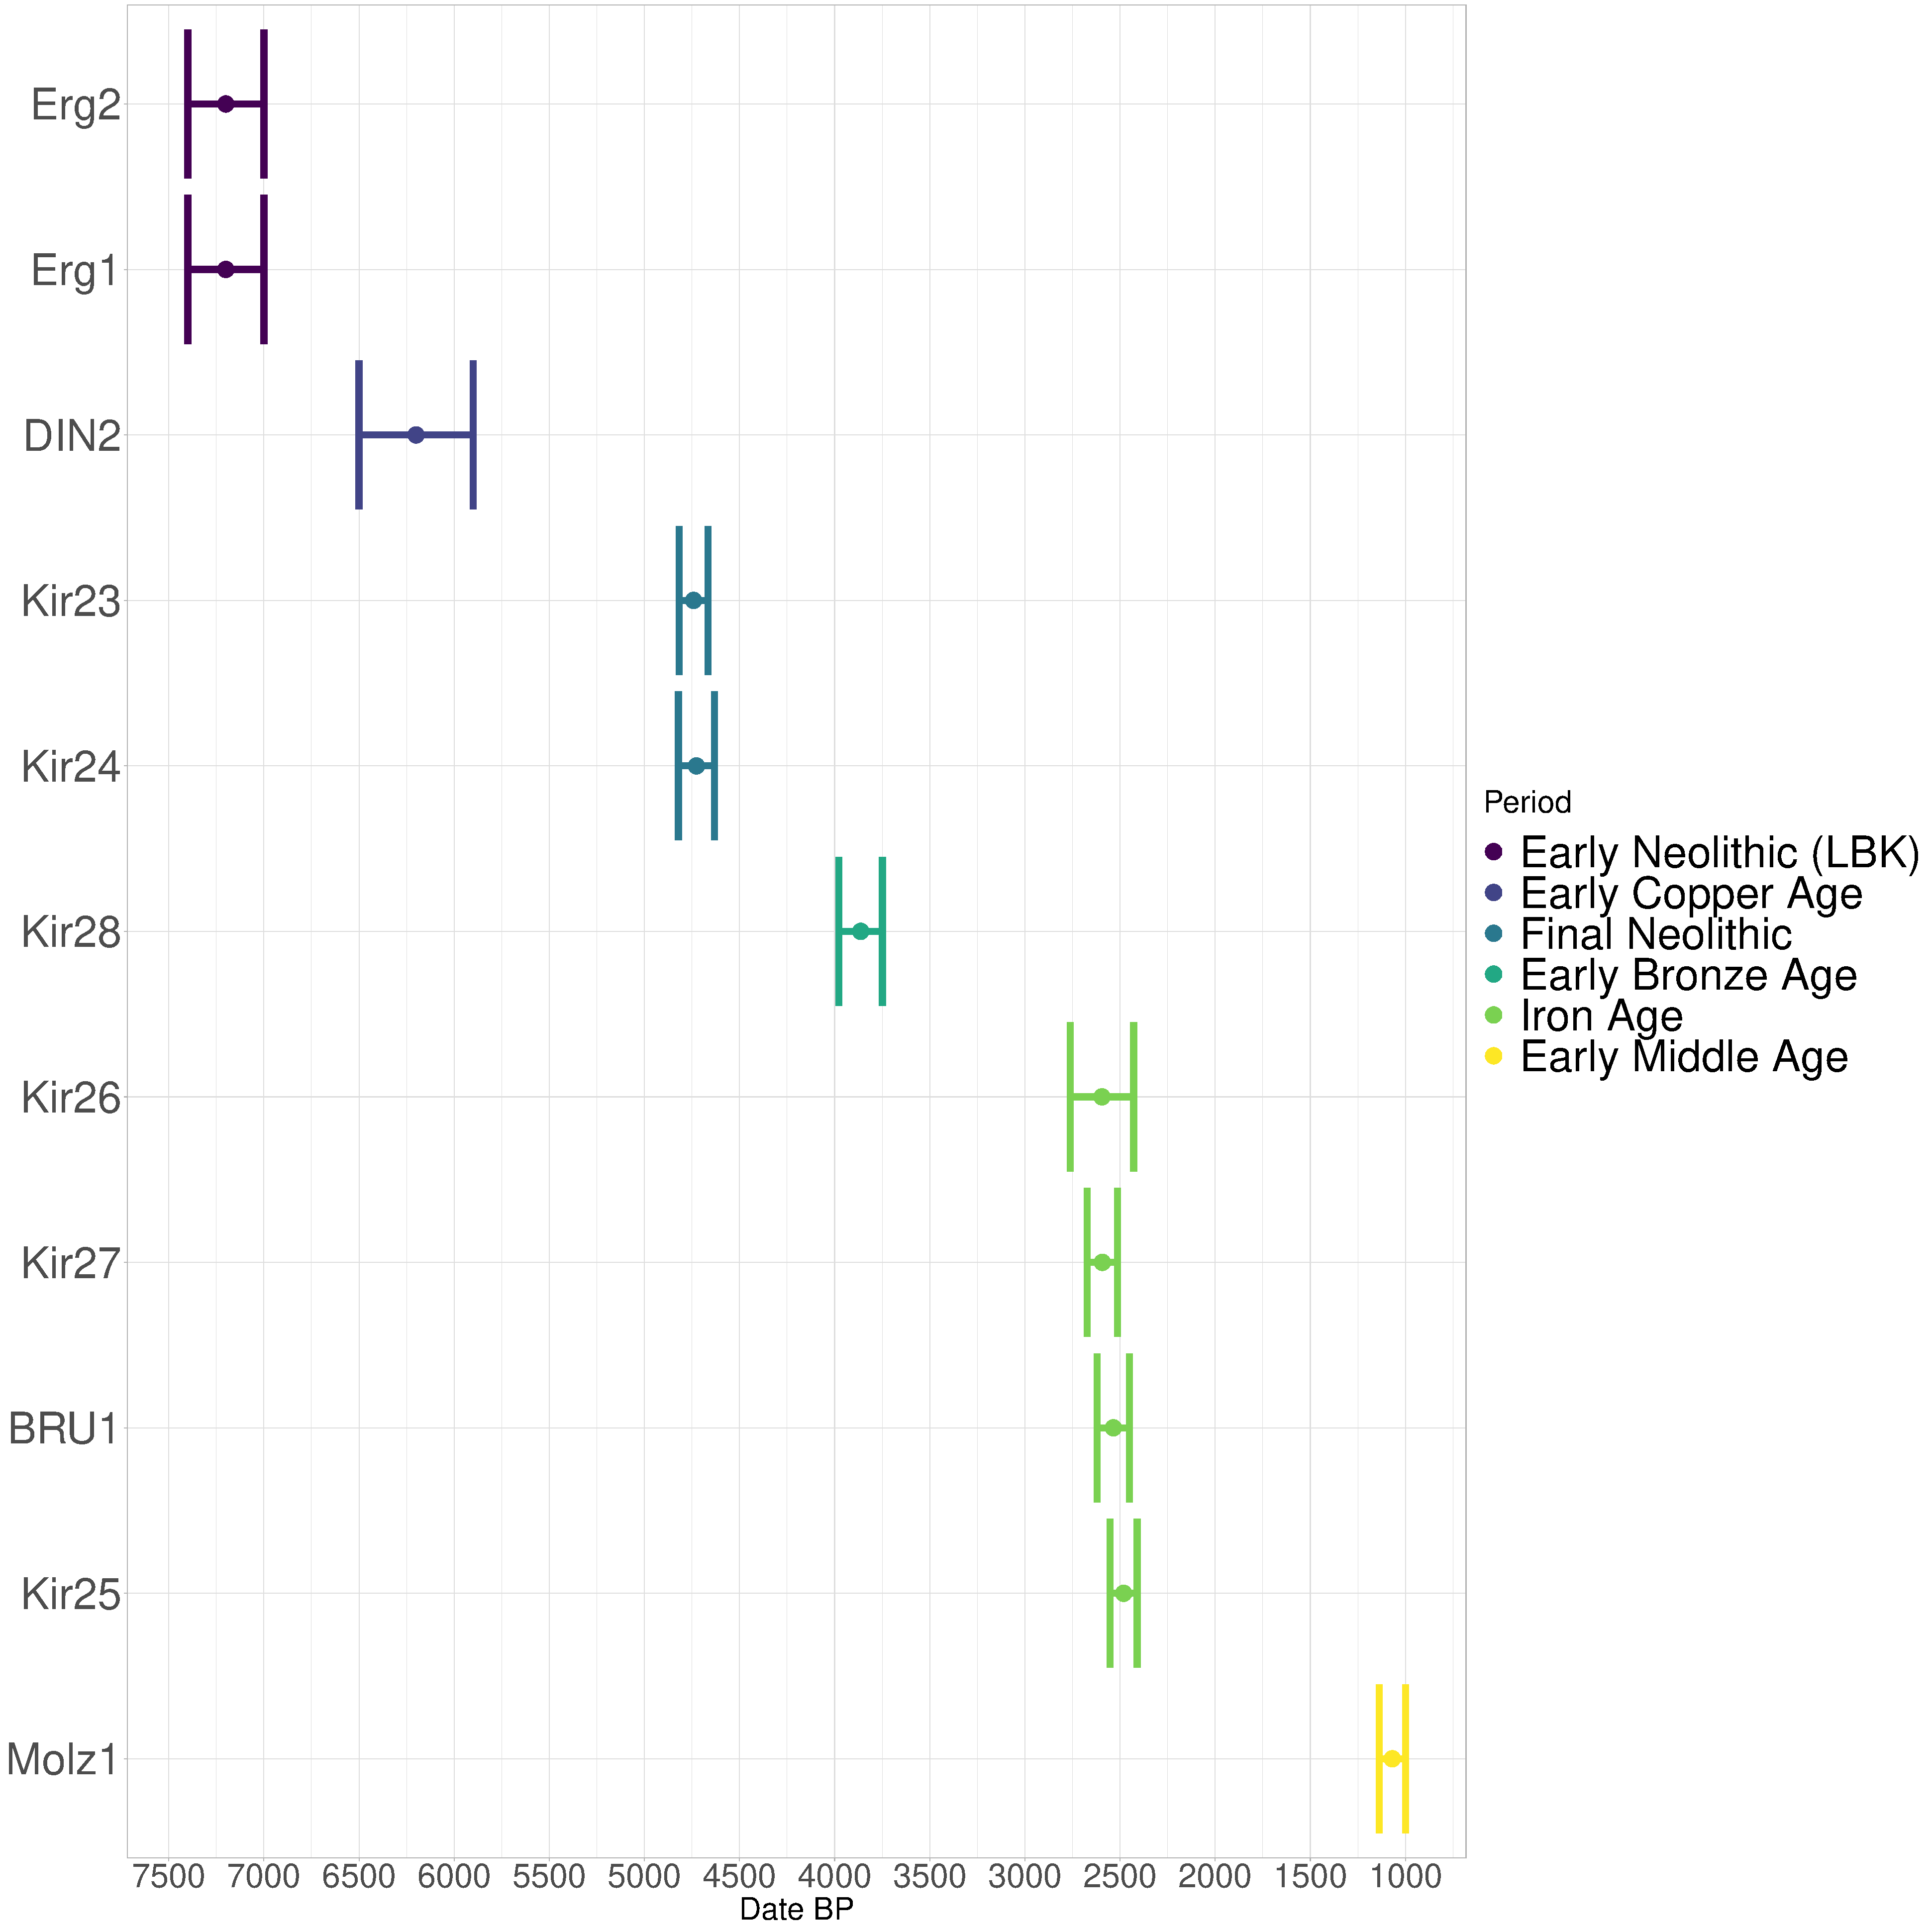
\includegraphics[width=1.0\textwidth]{../images/chapter4/Dates.pdf}
    \caption{Estimated radiocarbon dates for each newly sequenced ancient individual, grouped by archaeological period. Error bars correspond to upper and lower 95\% quantiles of the mean date.}
    \label{fig:chapter4_intro_SamplesDates}
\end{figure}

\begin{table}
\centering
\begin{tabular}[t]{llrrrlr}
\toprule
Sample.ID & Location & Date  & UQ  & LQ  & Period & \thead{Sequencing\\ Depth}\\
\midrule
Erg1 & Ergoldsbach & 5200 (BC) & 5400 & 5000 & Early Neo (LBK) & 4.52\\
Erg2 & Ergoldsbach & 5200 (BC) & 5400 & 5000 & Early Neo (LBK) & 0.71\\
DIN2 & Dingolfing & 4200 (BC) & 4500 & 3900 & Early Copper Age & 1.71\\
Kir24 & Cherry Tree Cave & 2762 (BC) & 2821 & 2632 & Final Neo & 3.98\\
Kir23 & Cherry Tree Cave & 2741 (BC) & 2817 & 2666 & Final Neo & 17.52\\
Kir28 & Cherry Tree Cave & 1863 (BC) & 1977 & 1749 & EBA & 17.30\\
Kir26 & Cherry Tree Cave & 595 (BC) & 762 & 428 & Iron Age & 4.84\\
Kir27 & Cherry Tree Cave & 593 (BC) & 672 & 514 & Iron Age & 16.60\\
BRU1 & Bruckberg & 535 (BC) & 620 & 450 & Iron Age & 11.54\\
Kir25 & Cherry Tree Cave & 481 (BC) & 552 & 410 & Iron Age & 4.55\\
Molz1 & Molzbichl & 1069 (AD) & 1138 & 1000 & Early Middle Age & 13.22\\
\bottomrule
\end{tabular}
\caption{Details of newly sequenced ancient DNA samples. UQ and LQ give upper and lower 95\% quantile estimates for radiocarbon dates. EBA is Early Bronze Age.}
\label{tab:BavariaSampleInfo}
\end{table}

\subsection{Genotype imputation and phasing using GLIMPSE}
\label{sssec:imputationphasingGLIMPSE}

In order to compare the genetic variation in the newly sequenced samples to a reference dataset, I merged them with the 942 ancient samples from the literature detailed in Appendix section \ref{section:AncientReferenceDataset}, resulting in a total of 955 samples in \texttt{.bcf} format with genotype likelihood data at 77,213,942 genome-wide SNPs. 

I followed the recommended GLIMPSE \cite{rubinacci2021efficient} imputation and phasing pipeline (\url{https://odelaneau.github.io/GLIMPSE/tutorial_b38.html}), using the 30x-coverage 1000 genomes dataset \cite{byrska2021high} as a reference panel. This resulted in phased haplotypes and posterior genotype likelihoods for each of the 955 individuals. 

\subsection{Uniparental haplogroups}

To determine the mtDNA haplogroups for each newly sequenced ancient sample, I used Haplogrep (\url{https://haplogrep.i-med.ac.at/}) \cite{weissensteiner2016haplogrep} on the raw \texttt{.fastq} file for each sample. 

\subsection{IBD sharing}

I used hap-IBD \cite{zhou2020fast} to estimate IBD segments greater than 2cM in length between all pairs of ancient individuals above 1.5x coverage (n=466), using the phased output from GLIMPSE as input haplotypes, the genetic maps  from (\url{http://bochet.gcc.biostat.washington.edu/beagle/genetic_maps/plink.GRCh37.map.zip}) and leaving all parameters as default. 

\subsection{plink PCA}

To obtain a broad overview of the ancestry of the newly sequenced individuals in the context of the 942 literature samples detailed in Appendix section \ref{section:AncientReferenceDataset}, I performed PCA on the pre-imputation genotypes using plink2 \cite{chang2015second}. Genotypes were set to missing in an individual if, at that position, they were covered by fewer than two reads. 

I retained the 500,000 markers with the lowest amount of missingness across all samples and LD-pruned the resulting SNPs using the settings \texttt{--maf 0.01} and \texttt{--indep-pairwise 50 5 0.2}. PCA was performed using default settings from plink2.

\subsection{ChromoPainter and fineSTRUCTURE analysis}

To characterise the ancestry of the newly sequenced ancient samples in the context of other ancient individuals, I first selected all newly sequenced samples and literature samples above 1.5x coverage (n=466) and performed an `all-v-all' painting where each sample was painted using all other samples. 1.5x was somewhat arbitrarily chosen as my previous work has shown this is a suitable threshold for the inclusion of samples for ChromoPainter analysis (section \ref{sec:ChromoPainterChap2}); whilst I show 0.5x as the cut-off for coverage-related effects, I chose to be conservative and opt for a higher threshold, given all but one of the 11 newly sequenced samples have average coverage $>1.5$x. I used this painting, hereafter referred to as `ancient' painting, to perform fineSTRUCTURE clustering and tree building on the ancient samples. 

I performed Principle Component Analysis on the coancestry matrix of the `ancients' painting using the \texttt{prcomp\_irlba} function from the irlba R library. To account for the fact that the diagonals of the coancestry matrix are always zeros (as an individual cannot be painted by themselves), I set the diagonal of each row to be the mean of that row, following Lawson et al 2012 \cite{Lawson2012}. Although there were 466 individuals in the `ancients' painting, not all of these were included in the chunklengths PCA. This was because many individuals in that set were not relevant to exploring the ancestry of the Bavarian individuals. For instance, when plotted, samples such as those from the Xiong Nu, a 3rd century BC culture from inner Mongolia, dominate the variation in a PCA to the point where identifying structure between the samples of interest becomes challenging. Therefore I removed 327 individuals based on visual inspection of the first two principal components.

\begin{table}
\centering
\begin{tabular}[t]{lc}
\toprule
Population & \thead{Number of\\samples}\\
\midrule
HB:belorussian & 9\\
HB:bulgarian & 31\\
HB:croatian & 19\\
HB:cypriot & 12\\
HB:french & 28\\
HB:german & 30\\
HB:germanyaustria & 4\\
HB:greek & 20\\
HB:hungarian & 19\\
HB:irish & 7\\
HB:lithuanian & 10\\
HB:mordovian & 15\\
HB:northitalian & 12\\
HB:norwegian & 18\\
HB:polish & 17\\
HB:romanian & 16\\
HB:russian & 25\\
HB:scottish & 6\\
HB:siciliane & 10\\
HB:southitalian & 18\\
HB:spanish & 34\\
HB:tsi & 98\\
HB:tuscan & 8\\
HB:ukrainian & 20\\
HB:welsh & 4\\
HB:westsicilian & 10\\
\bottomrule
\end{tabular}
\caption{Name of population and number of samples used in the present-day ChromoPainter, MOSAIC and qpAdm analyses. All populations from the HellBus dataset.}
\label{tab:BavariaModernSamples}
\end{table}

To determine the genetic similarity between the newly sequenced ancient samples and present-day populations, I performed an `all-v-all' painting using a selected group of 26 present-day European populations (Table \ref{tab:BavariaModernSamples}) from the HellBus dataset (described in Appendix section \ref{section:MSPOBIHellBus}) and the 11 newly sequenced ancient individuals, hereafter referred to as `present-day painting'.

I applied fineSTRUCTURE (v0.0.5)\cite{Lawson2012} to cluster the chunkcounts ChromoPainter output for the `ancients' painting. fineSTRUCTURE assigns individuals to clusters, estimates the  number of clusters and builds a dendrogram of genetic similarity based on a tree-building algorithm. This is particularly useful when combining many samples from different studies, as is the case with the `ancients' painting; the population label identifiers used by different studies may not be consistent with one another. Therefore, we can use fineSTRUCTURE groupings as population labels rather than group labels. fineSTRUCTURE was first run in MCMC mode using 1,000,000 burn-in MCMC iterations and 2,000,000 main MCMC iterations. It was then run in tree-building mode (\texttt{-m T}) using 100,000 burn-in and 100,000 main iterations. 

Tree figures, coancestry matrix figures and principle component plots were generated using the fineSTRUCTURE R library \url{(https://people.maths.bris.ac.uk/~madjl/finestructure/FinestructureRcode.zip)}.

\subsection{SOURCEFIND} \label{sec:ch4_SOURCEFIND}

I used SOURCEFIND \cite{Chacon-Duque2018} to infer the proportions of ancestry by which each newly sequenced ancient individual is most related to a set of surrogate populations. While this method does not explicitly attempt to identify admixture, in contrast to e.g. ALDER \cite{LohAlderAdmixture} or GLOBETROTTER \cite{Hellenthal2014}, it can reflect admixture proportions \cite{Chacon-Duque2018} but more generally reflects recent ancestry sharing patterns.

The first analysis used the ancients painting and only three surrogates: Western Hunter-Gatherers, Neolithic farmers from Anatolia and Yamnaya, to mimic previous research suggesting many ancient Europeans descend from the mixture of three sources well-represented by these groups \cite{Lazaridis2014}. The second analysis attempted to characterise more fine-scale ancestry patterns, by modelling each target ancient individual (using the same ancients painting) as a mixture of all sampled ancient populations above 1.5x coverage (n=466) that had an average sample age no more than 100 years younger than that of the target individual. The third analysis used the ``modern'' painting and formed each ancient individual as a mixture of all present-day populations shown in Table \ref{tab:BavariaModernSamples}. For each of these analyses, I found the mean and 95\% credible interval of ancestry estimates across 2,000,000 posterior samples combined from three independent SOURCEFIND runs that each sampled every 10,000 MCMC iterations after discarding the first 10,000 MCMC iterations as ``burn-in''.


\subsection{MOSAIC admixture analysis}

I inferred admixture events, dates and proportions in newly sequenced ancient samples using MOSAIC, a haplotype-based method \cite{MOSAIC_2019}. While MOSAIC cannot infer multiple pulses of admixture from the same admixing sources as GLOBETROTTER \cite{Hellenthal2014} can, in theory it is unlikely we would have adequate power to identify such multiple pulses when analysing only a single ancient sample, as is the case in this study. Furthermore, the `painting' step and admixture inference step in MOSAIC are combined, providing a simpler pipeline and more flexible assignment of different surrogates relative to GLOBETROTTER (i.e.\ the set of surrogates can be changed without repainting the samples).

I performed two MOSAIC analyses that correspond to two of the SOURCEFIND analyses described in Section \ref{sec:ch4_SOURCEFIND}. First, I performed an `ancient surrogates' analysis where the all ancient samples above 1.5x coverage (n=466) were used as surrogates to admixing sources. I used the fineSTRUCTURE groupings to categorise ancient samples into surrogate populations. Second, I also performed a `present-day surrogates' analysis where a selected set of present-day populations (Table \ref{tab:BavariaModernSamples}) were used as surrogates. While using present-day populations to reflect ancestry patterns in ancient individuals may be counter-intuitive, the larger sample sizes and larger variety of present-day populations can provide more clean results relative to using ancients

I ran MOSAIC using default settings, assuming two or three admixing sources per target individual/population. For populations with more than one sampled individual, MOSAIC provided bootstrap-based 95\% confidence quantiles around date estimates. MOSAIC also estimates $f_{st}$ between the set of surrogates and the estimated `true' mixing source, which is useful when a close proxy for the `true' mixing source is not available

\subsection{F-statistics}

Many of the relevant samples in the literature were of very low coverage ($<0.1$). As my work in section \ref{sec:ChromoPainterChap2} indicated that samples with less than 0.5x coverage cannot reliably be analysed using ChromoPainter, I also used F-statistics \cite{Patterson2012} that are mostly robust to coverage related effects \cite{AssessingqpAdm}. In particular I used Admixtools \url{(https://uqrmaie1.github.io/admixtools)} to analyse 942 individuals from 143 populations (Appendix section \ref{section:AncientReferenceDataset}, including many low-coverage samples from relevant LBK cultures presented in Rivollat et al (2020) that would not have been suitable for use with ChromoPainter \cite{rivollat2020france}. This analysis also incorporated 2280 present-day individuals from 144 populations from the HellBus dataset as putative ancestry surrogates for tested ancient individuals. Populations shown in Table \ref{tab:BavariaModernSamples}. 

For the input to ADMIXTOOLS, I used the genotyped imputed from GLIMPSE, as it has been shown that using imputed markers reduced reference bias relative to using pseudo-haploid markers \cite{Martiniano2017}. I then used the $f_{4}$ branch test to test whether two populations form a clade relative to two other populations. For example, the expected value of $f_{4}(french,german;yoruba,mbuti)$, which tests whether \{french,german\} form a clade relative to \{yoruba,mbuti\}, should not give a score significantly different to zero. In contrast, exchanging $french$ with $yoruba$ would yield a significantly positive $f_4$ scores, with strength of evidence to reject the null ($f_4 = 0$) measured using standardised $Z$-statistics.

I also used the $f_3$ test, denoted $f_{3}(A,B;C)$, to (i) estimate the branch length between $A$ and $B$ after their divergence from $C$, or (ii) test whether $C$ descends from an admixture event between sources represented by $A$ and $B$. The latter can occur if $C$ has a substantial number of SNPs with allele-frequencies which are intermediate between $A$ and $B$.

Finally, I used qpAdm to infer ancestry proportions, following the protocol described in Olalde et al (2018) by choosing the following populations/samples as outgroups: \textit{Mota}, \textit{Kostenki14}, \textit{papuan}, \textit{han}, \textit{hannchina}, \textit{mbutipygmy}, \textit{sannamibia}, \textit{yakut}. These outgroups were suitable for use in investigating ancient Eurasians, since they are asymmetrically related to many ancient populations, but do not show evidence of recent gene flow with them. 

\section{Results}

\subsection{Broad-scale ancestry changes in Bavaria reflect those found elsewhere in Europe}

The newly sequenced samples from the Early Neolithic (Erg1 and Erg2, approx 5200BC) and Copper Age (DIN2, approx 4200BC) cluster with other literature samples from European Neolithic on the plink2 PCA (Fig. \ref{fig:plink_PCA}). As in previously reported PCA results \cite{Lipson2017b}, the earliest Neolithic samples, from Anatolia and Greece, and who are thought to be the source population from which all subsequent Neolithic farmers derive \cite{Hofmanova2016, Haak2010, haak2005ancient, bramanti2009genetic, Lazaridis2014}, are  positioned at the end of the cluster farthest away from the hunter-gatherer samples (for example, WHG on Fig. \ref{fig:plink_PCA}). This likely reflects the fact that they are unadmixed with respect to the later Neolithic samples. As the Neolithic progressed, farmers from the near-east mixed with local hunter-gatherer groups in central Europe \cite{Lipson2017b} and acquired local hunter-gatherer ancestry. Accordingly, these samples are shifted away from the earlier Neolithic samples towards the hunter-gatherers. With this in mind, the position of the new Early Neolithic sample Erg1, shifted north away from the contemporaneous sample Erg2, is suggestive of hunter-gatherer admixture. 

There are four key observations from the Figure \ref{fig:plink_PCA} PCA regarding the new samples:

\begin{enumerate}
\item The two Late Neolithic individuals are genetically separate, with Kir24 positioned close to Yamnaya and Kir23 clustering with Neolithic Europeans.
\item The Bronze Age sample Kir28 clusters with other European Bronze Age samples
\item The four Iron Age samples (Kir25, Kir26, Kir27 and BRU1) cluster towards the Neolithic individuals and other European Iron Age samples
\item The three Medieval period samples (Alh1, Alh10, Molz1) cluster with the Bronze Age sample Kir28 instead of the Iron Age samples.
\end{enumerate}

\begin{figure}[htp]
    \centering
    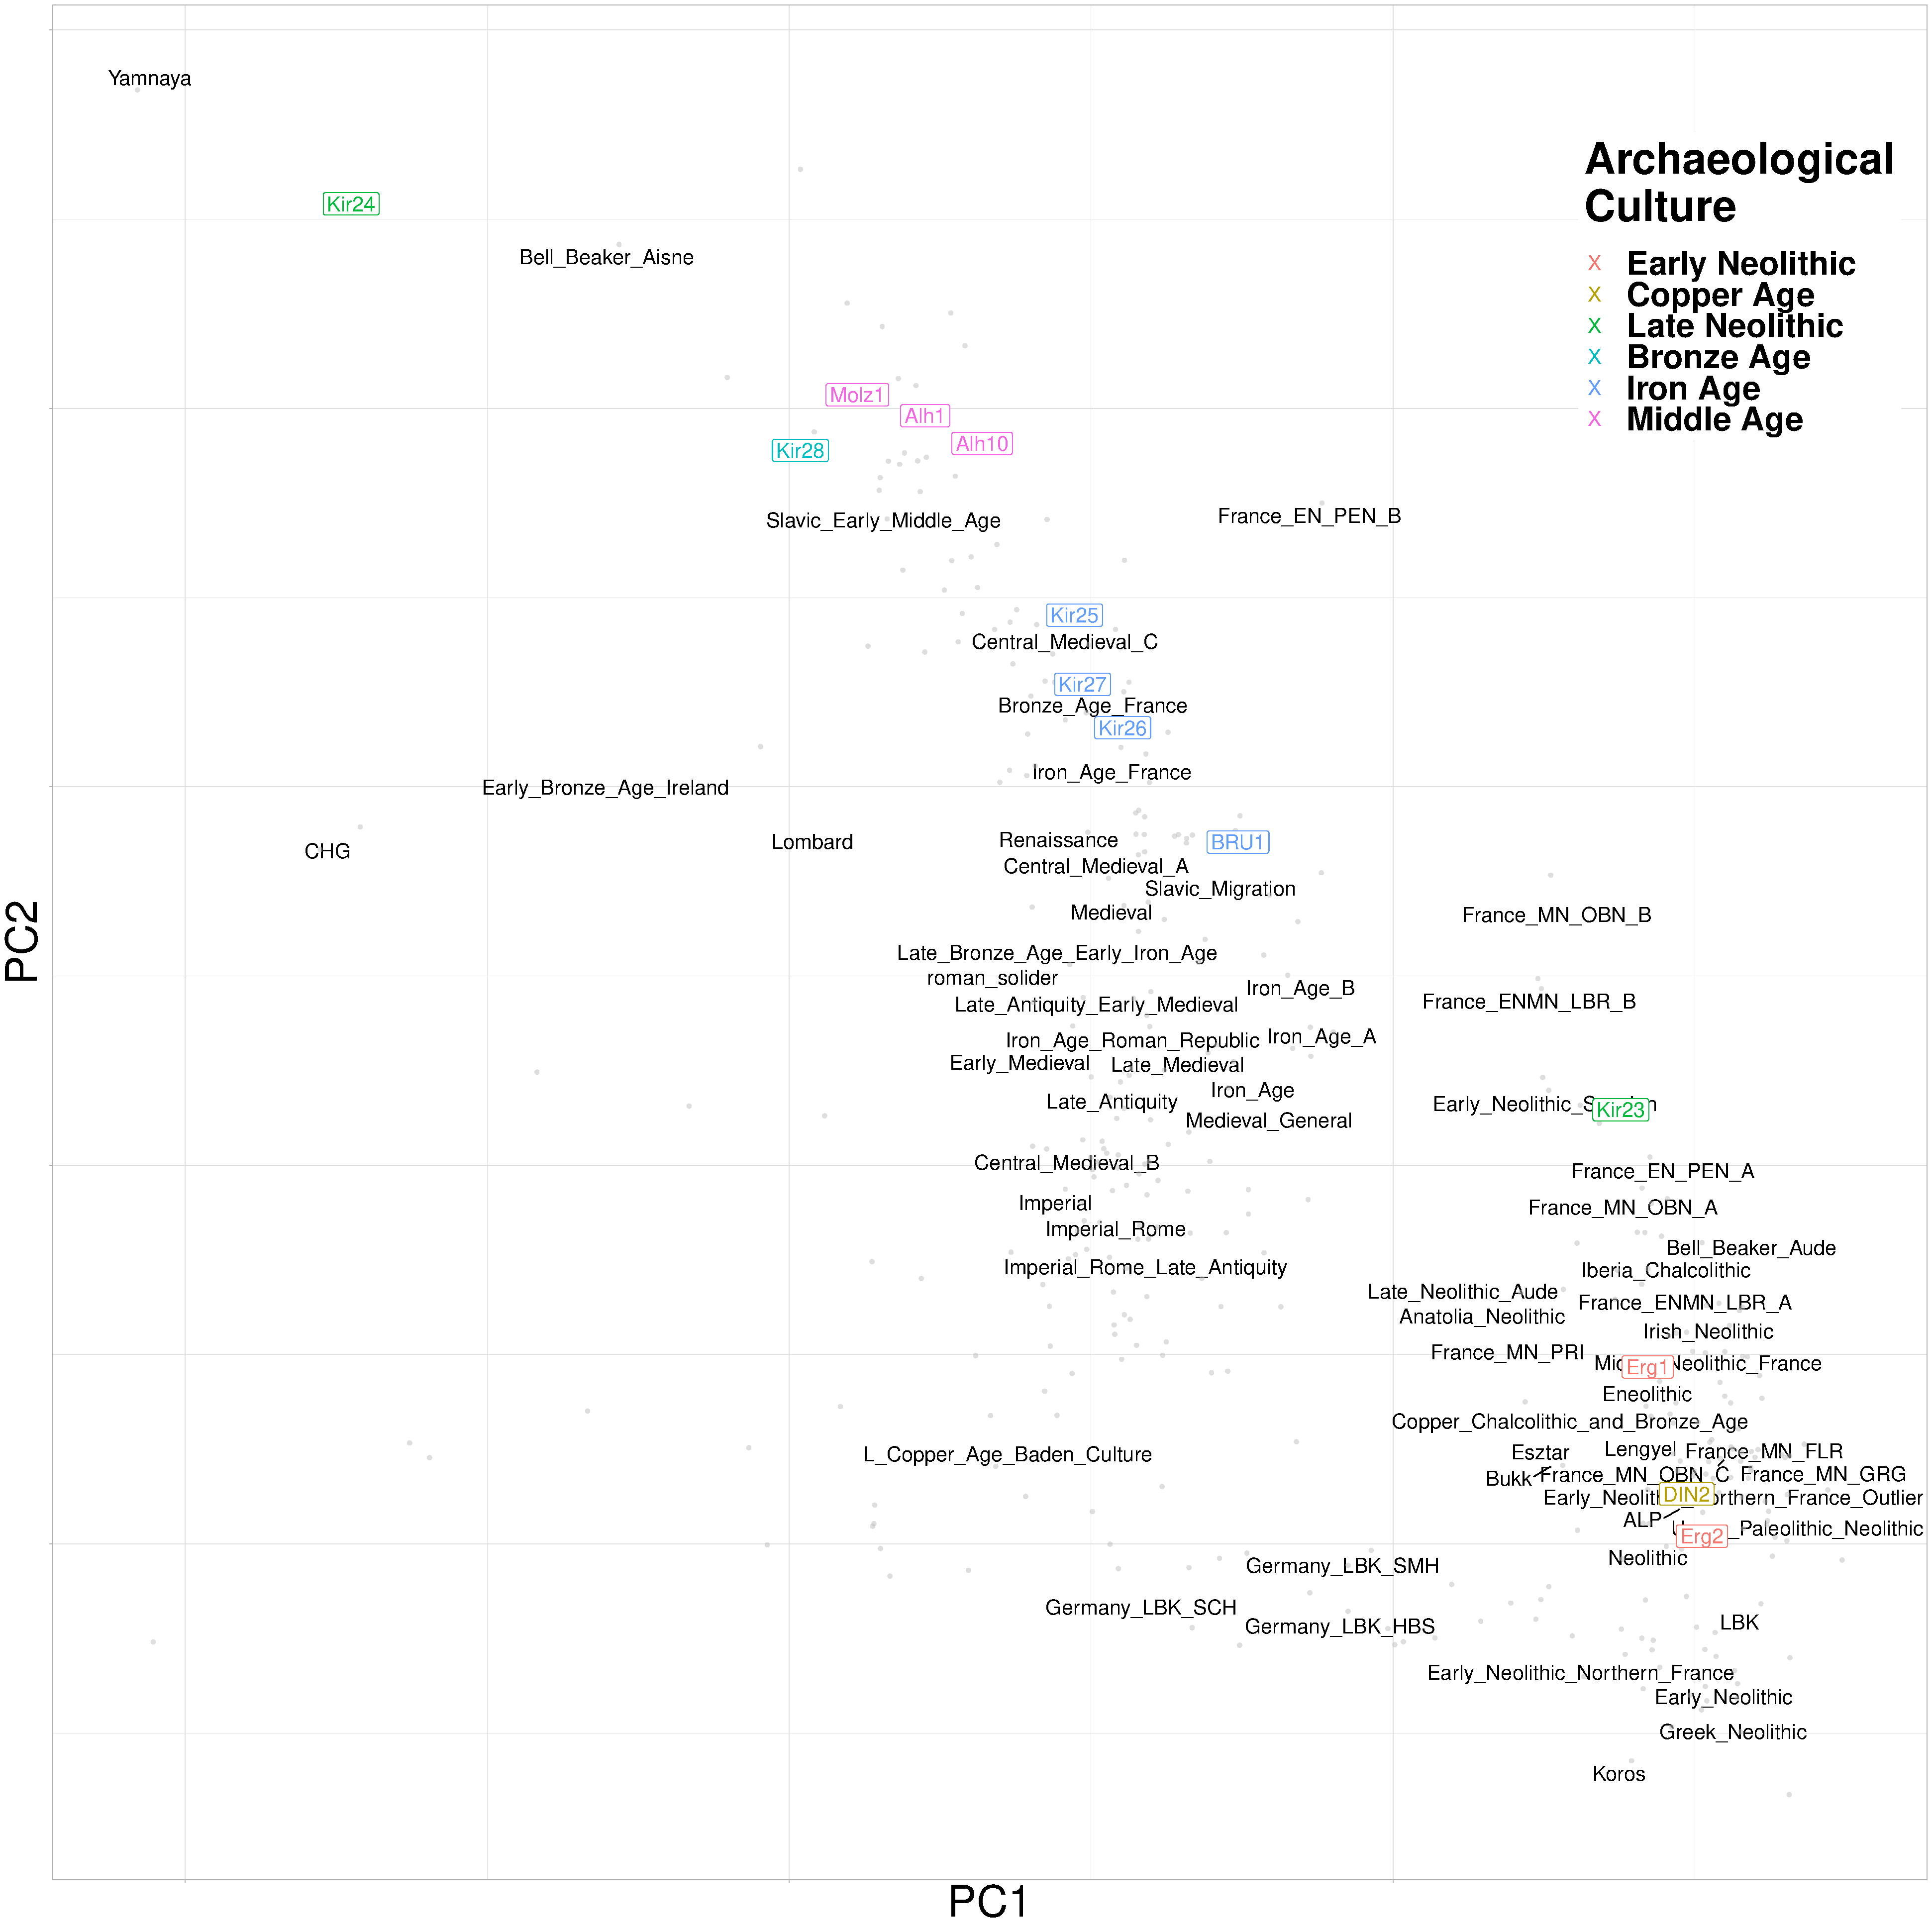
\includegraphics[width=1.0\textwidth]{../images/chapter4/plink_PCA.pdf}
    \caption{Principle component analysis of pre-imputation genotypes using plink2. Grey points indicate principle component coordinates for each sample. Black text indicated mean principle component coordinates for all individuals within that group. Coloured labels represent newly sequenced ancient samples.}
    \label{fig:plink_PCA}
\end{figure}

\subsection{Early Neolithic}

\begin{figure}[htp]
    \centering
    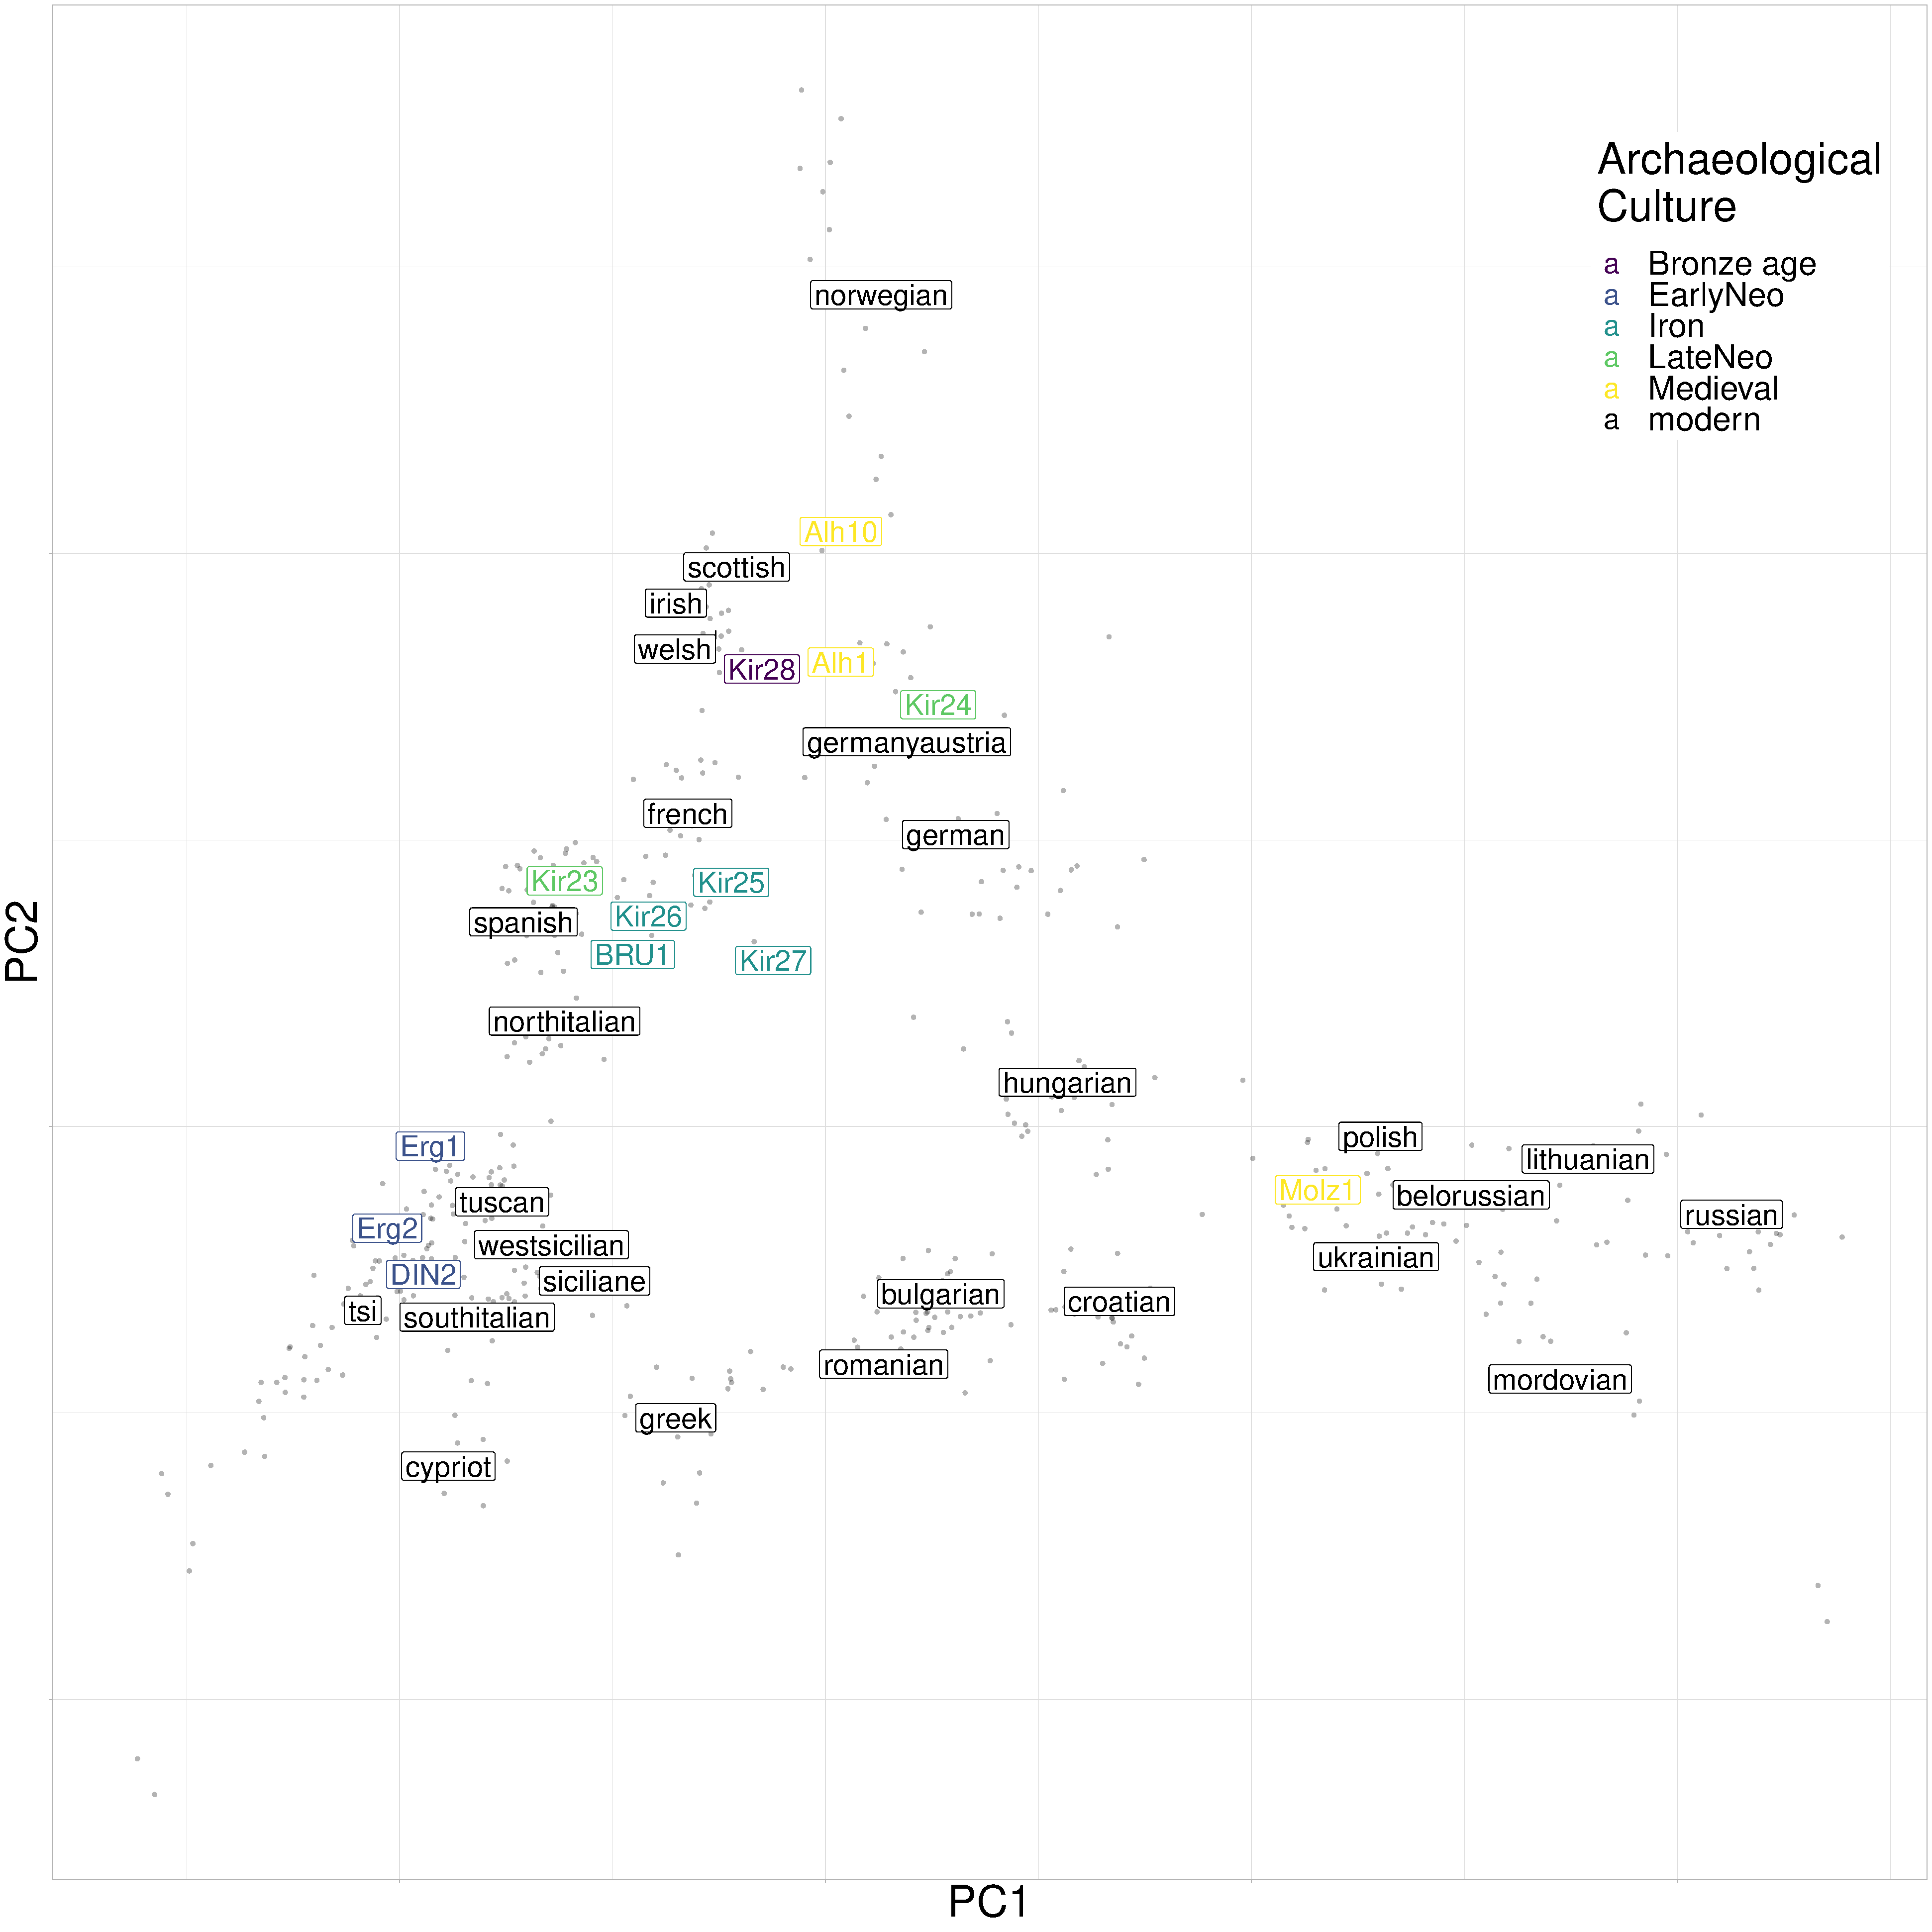
\includegraphics[width=1.0\textwidth]{../images/chapter4/chunklengths_moderns_ancients_PCA.pdf}
    \caption{Principle component plot of newly sequenced ancient samples and reference modern individuals performed using the finestructure library. Green labels correspond to Migration Era samples, red labels correspond to Early Middle Age samples and white labels correspond to reference populations. The position of each reference label is the mean PC coordinates of all individuals within that population. Transparent coloured points correspond to present-day individuals.}
    \label{fig:chunklengths_moderns_ancients_PCA_bav}
\end{figure}

The three Early/Middle Neolithic samples, Erg1, Erg2 and DIN2, all display a strong affinity to Anatolian farmers, consistent with the prevailing theory that near-eastern farmers were responsible for the spread of early agricultural technology across Europe, and that all Neolithic farmers share recent common ancestry \cite{Haak2010, haak2005ancient, bramanti2009genetic, Lazaridis2014}. fineSTRUCTURE  grouped Erg1 with two samples from Upper Palaeolithic/Neolithic Italy and DIN2 with Early/Middle Neolithic samples from Germany, Greece, Anatolia and Hungary. Despite their age, the genetic variation of the Early Neolithic samples falls well within the variation of present-day individuals; when painted using present-day samples, the three Early Neolithic individuals cluster with present-day Italians, consistent with findings from previous research \cite{Lazaridis2014, Haak2015} (Fig. \ref{fig:chunklengths_moderns_ancients_PCA_bav}). Erg1 was assigned to mtDNA haplogroup K which has been found in Neolithic and pre-pottery sites across Europe \cite{Hofmanova2016, fernandez2014ancient} and Western Asia \cite{Lazaridis2016, Mathieson2015}. 

Erg1 is from the \textit{Linearbandkeramik} (LBK) culture and is speculated to have belonged to the first wave of immigrants carrying farming technology from south-eastern Europe or Anatolia into central Europe. DIN2 is from a nearby site, around 500 years more recent, and is thought to potentially belong to a second wave of farmers who migrated along the Danube. It is unclear to what extent these different waves corresponded to populations with different ancestries.  

When painted using 465 ancient samples from the literature and the newly sequenced samples, Erg1 had the lowest $TVD$ ($TVD$ is a distance metric based on ChromoPainter copyvectors; calculation and justification outlined in Appendix section \ref{sec:appendixTVD}) with DIN2, supporting the hypothesis that they were from similar source population. DIN2  has the lowest $TVD$ with NE5, NE4 and NE7, samples assigned to Middle and Late Neolithic cultures on the Hungarian plane, and was assigned to mitochondrial haplogroup (J1C) alongside NE4 and NE5. Both the autosomal and mtDNA link to Neolithic Hungary supports the hypothesis that DIN2 migrated along the Danubian route.   

To explicitly test whether Erg1 and DIN2 group together to the exclusion of other ancient samples and therefore, whether they likely originated from a similar source population, I performed $f_{4}$ tests in the form of $f_{4}(W=Erg1, X=DIN2; Y=test, Z=Mbuti)$, where $test$ is 143 ancient populations used in the F-statistics analysis. This tests whether Erg1 and DIN2 form a clade to the exclusion of $test$ or not. Of the 143 comparisons, only the population labelled as WHG had a $|Z|>3$, ($Z=3.057$), suggesting that Erg1 and DIN2 originate from the same local population. Note that one test with $|Z|>3$ may be expected when doing 143 tests, even if the null is true.

To determine whether Erg1 showed increased genetic similarity to local farming populations, I also performed combinations of $f_{3}$ in the form of $f_{3}(A=Erg1, B=test, C=Mbuti)$, where $test$ iterates across 143 ancient populations. This tests the branch length, or the amount of genetic drift that has occurred on the branch shared by Erg1 and $test$ since their divergence from an outgroup (Mbuti). The sample/population with the highest $f_{3}$ statistic was NE7, a sample from 4,360 – 4,490 BC and the Lengyel culture (a Neolithic culture centered on the Danube River, known to be an offshoot of the LBK culture Erg1 belonged to). On the other hand, DIN2 shows a clear affinity to samples from Neolithic France.

My dataset included data from several other LBK populations local to Erg1 and DIN2; samples from Schwetzingen, Stuttgart-Mullhausen and Halberstadt. These samples appear to form a distinct cluster on the plink PCA and are shifted away from the primary cluster of Neolithic individuals and towards samples from the Anatolian Bronze Age and Baden Culture (a central European Chalcolithic culture) (Fig. \ref{fig:plink_PCA}). I wanted to know which LBK population Erg1 and DIN2 were closest to. I found strong evidence ($|Z| = 7.97$) that Erg1 shared more alleles with LBK populations from Schwetzingen than with Stuttgart-Mühlhausen, suggesting the early LBK populations showed relatively fine-scale geographic structure. Given the lack of Hunter Gatherer ancestry in the Rivollat LBK samples, this structure seems unlikely to be driven by variable amounts of Hunter-Gatherer admixture (Fig. \ref{fig:HG_ancestry_Neolithic}).


\subsection{Variable amounts of local hunter-gather ancestry in Neolithic farmers indicates a structured population}

Prior research has shown that admixture occurred between newly arrived farming immigrants from Anatolia and local hunter-gatherers \cite{Gamba2014, Haak2015, mathieson2018genomic, gonzalez2017paleogenomic, Lipson2017b}. The position of Erg1 on the PCA, shifted slightly north towards the majority of the Bronze Age samples, suggests that it may have a component of Hunter-Gatherer ancestry. Indeed an $f_{3}$ admixture test, using $f_{3}(A=Castelnovian Mesolithic, B=LBK; C=Erg1)$ to test for admixture in $C$ from two sources related to surrogates $A$ and $B$, yielded a significantly negative result $(|Z|=4.25)$, as expected in the case of admixture \cite{Patterson2012}. Furthermore, qpAdm also concluded that Erg1 can be modelled as a mixture of Anatolia Neolithic (66\%, se=8.1) and WHG (33\%, se=8.1). In contrast, qpAdm modelled Erg2 as descending solely from sources related to Anatolian Neolithic farmers. MOSAIC also inferred admixture in Erg1, dated to 5.3 generations prior to it sample date (i.e. approximately 5288 years ago), between WHG and Anatolia Neolithic sources. I caution that the admixture date may be unreliable due to only targeting a single individual, and given MOSAIC bootstraps over individuals, it was not possible to obtain confidence intervals around admixture date. 

\begin{figure}[htp]
    \centering
    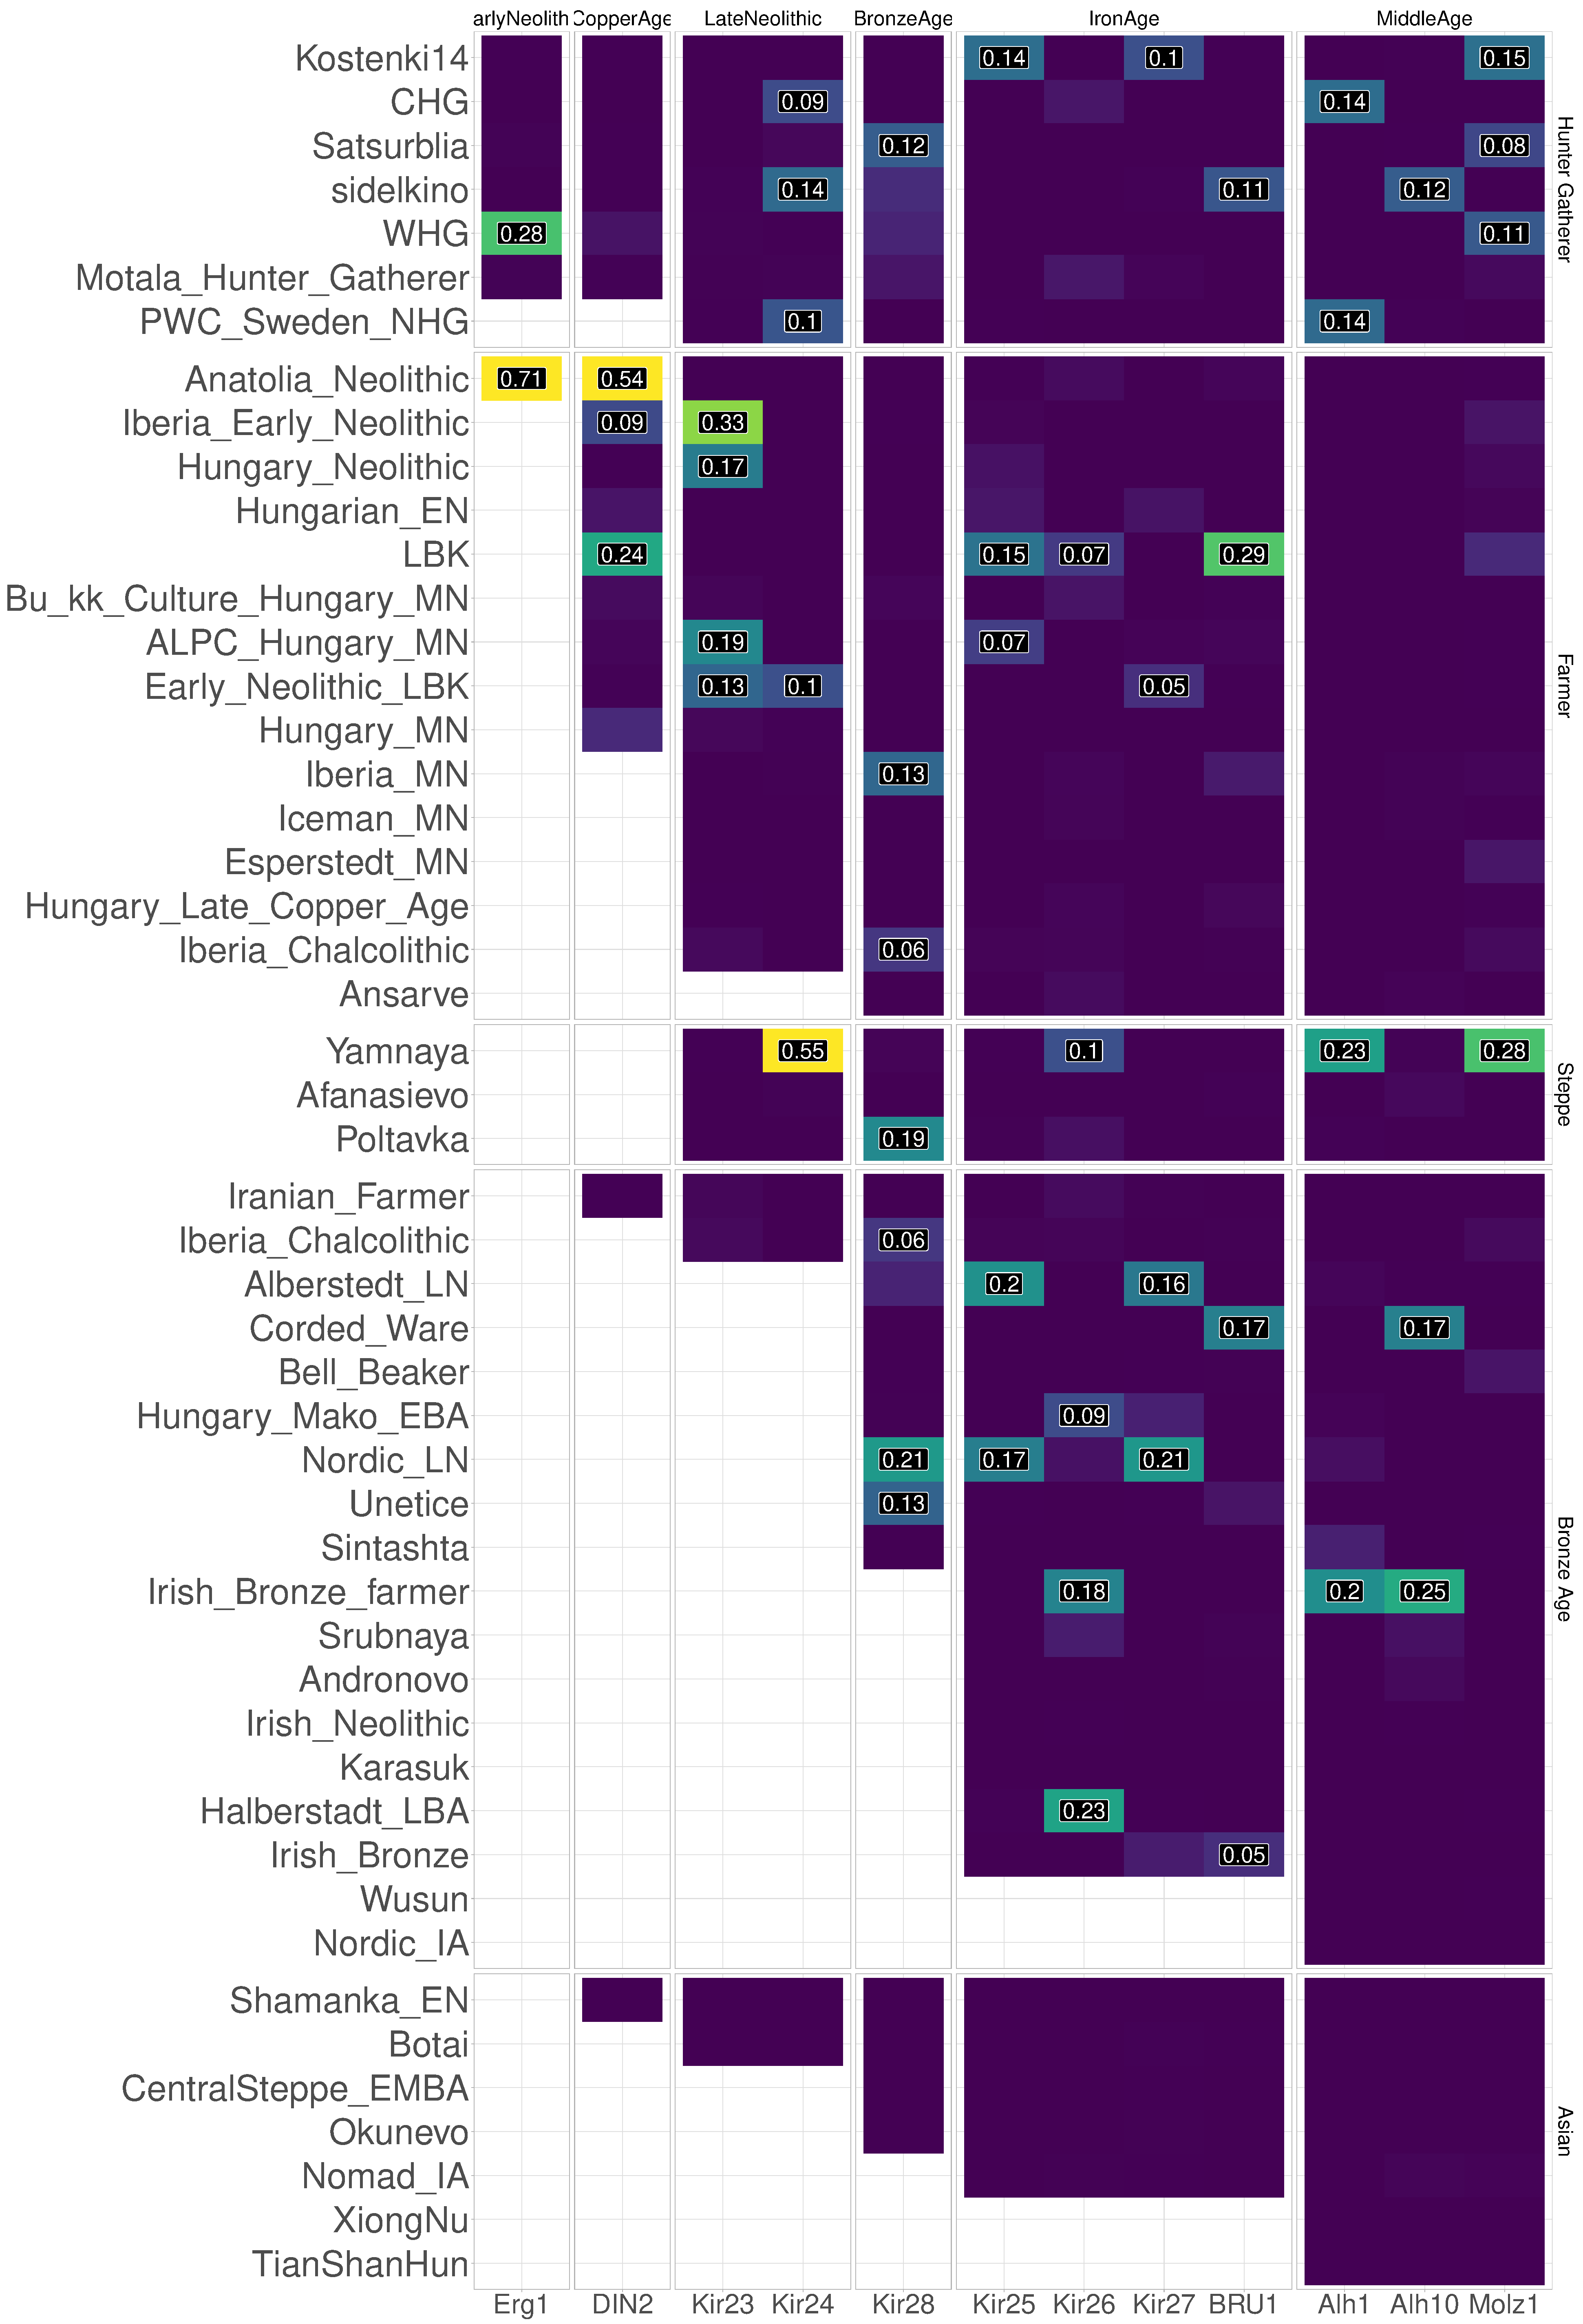
\includegraphics[width=1.0\textwidth]{../images/chapter4/SOURCEFINDheatmapOlderSurrogates_2.pdf}
    \caption{SOURCEFIND ancestry proportion estimates for all newly sequenced target samples (vertical columns). Target samples are grouped by archaeological age. Surrogate populations are represented as horizontal rows and also grouped into archaeological culture. Each target was modeled as a mixture of only populations which are dated to being older or contemporaneous as the the target. Numbers within each cell correspond to the ancestry proportion estimate.}
    \label{fig:chapter4resultsSFheatmapolder}
\end{figure}


Estimated Hunter-gatherer related ancestry in Erg1 ranged from 18-38\% among MOSAIC, qpAdm, with SOURCEFIND inferring 27.2\% (se=1.41) when using six surrogates \{Anatolian Neolithic, Loschbour, LaBrana, Bichon, and the two `Iron Gates' samples\}. MOSAIC indicated the cluster of Italian hunter-gatherers as the closest population to the true mixing source (Fig. \ref{fig:Erg1_MU_matrix}). However, SOURECFIND indicated Iron Gates individuals from Serbia as the largest contributors of hunter-gatherer related ancestry.


\begin{figure}[htp]
    \centering
    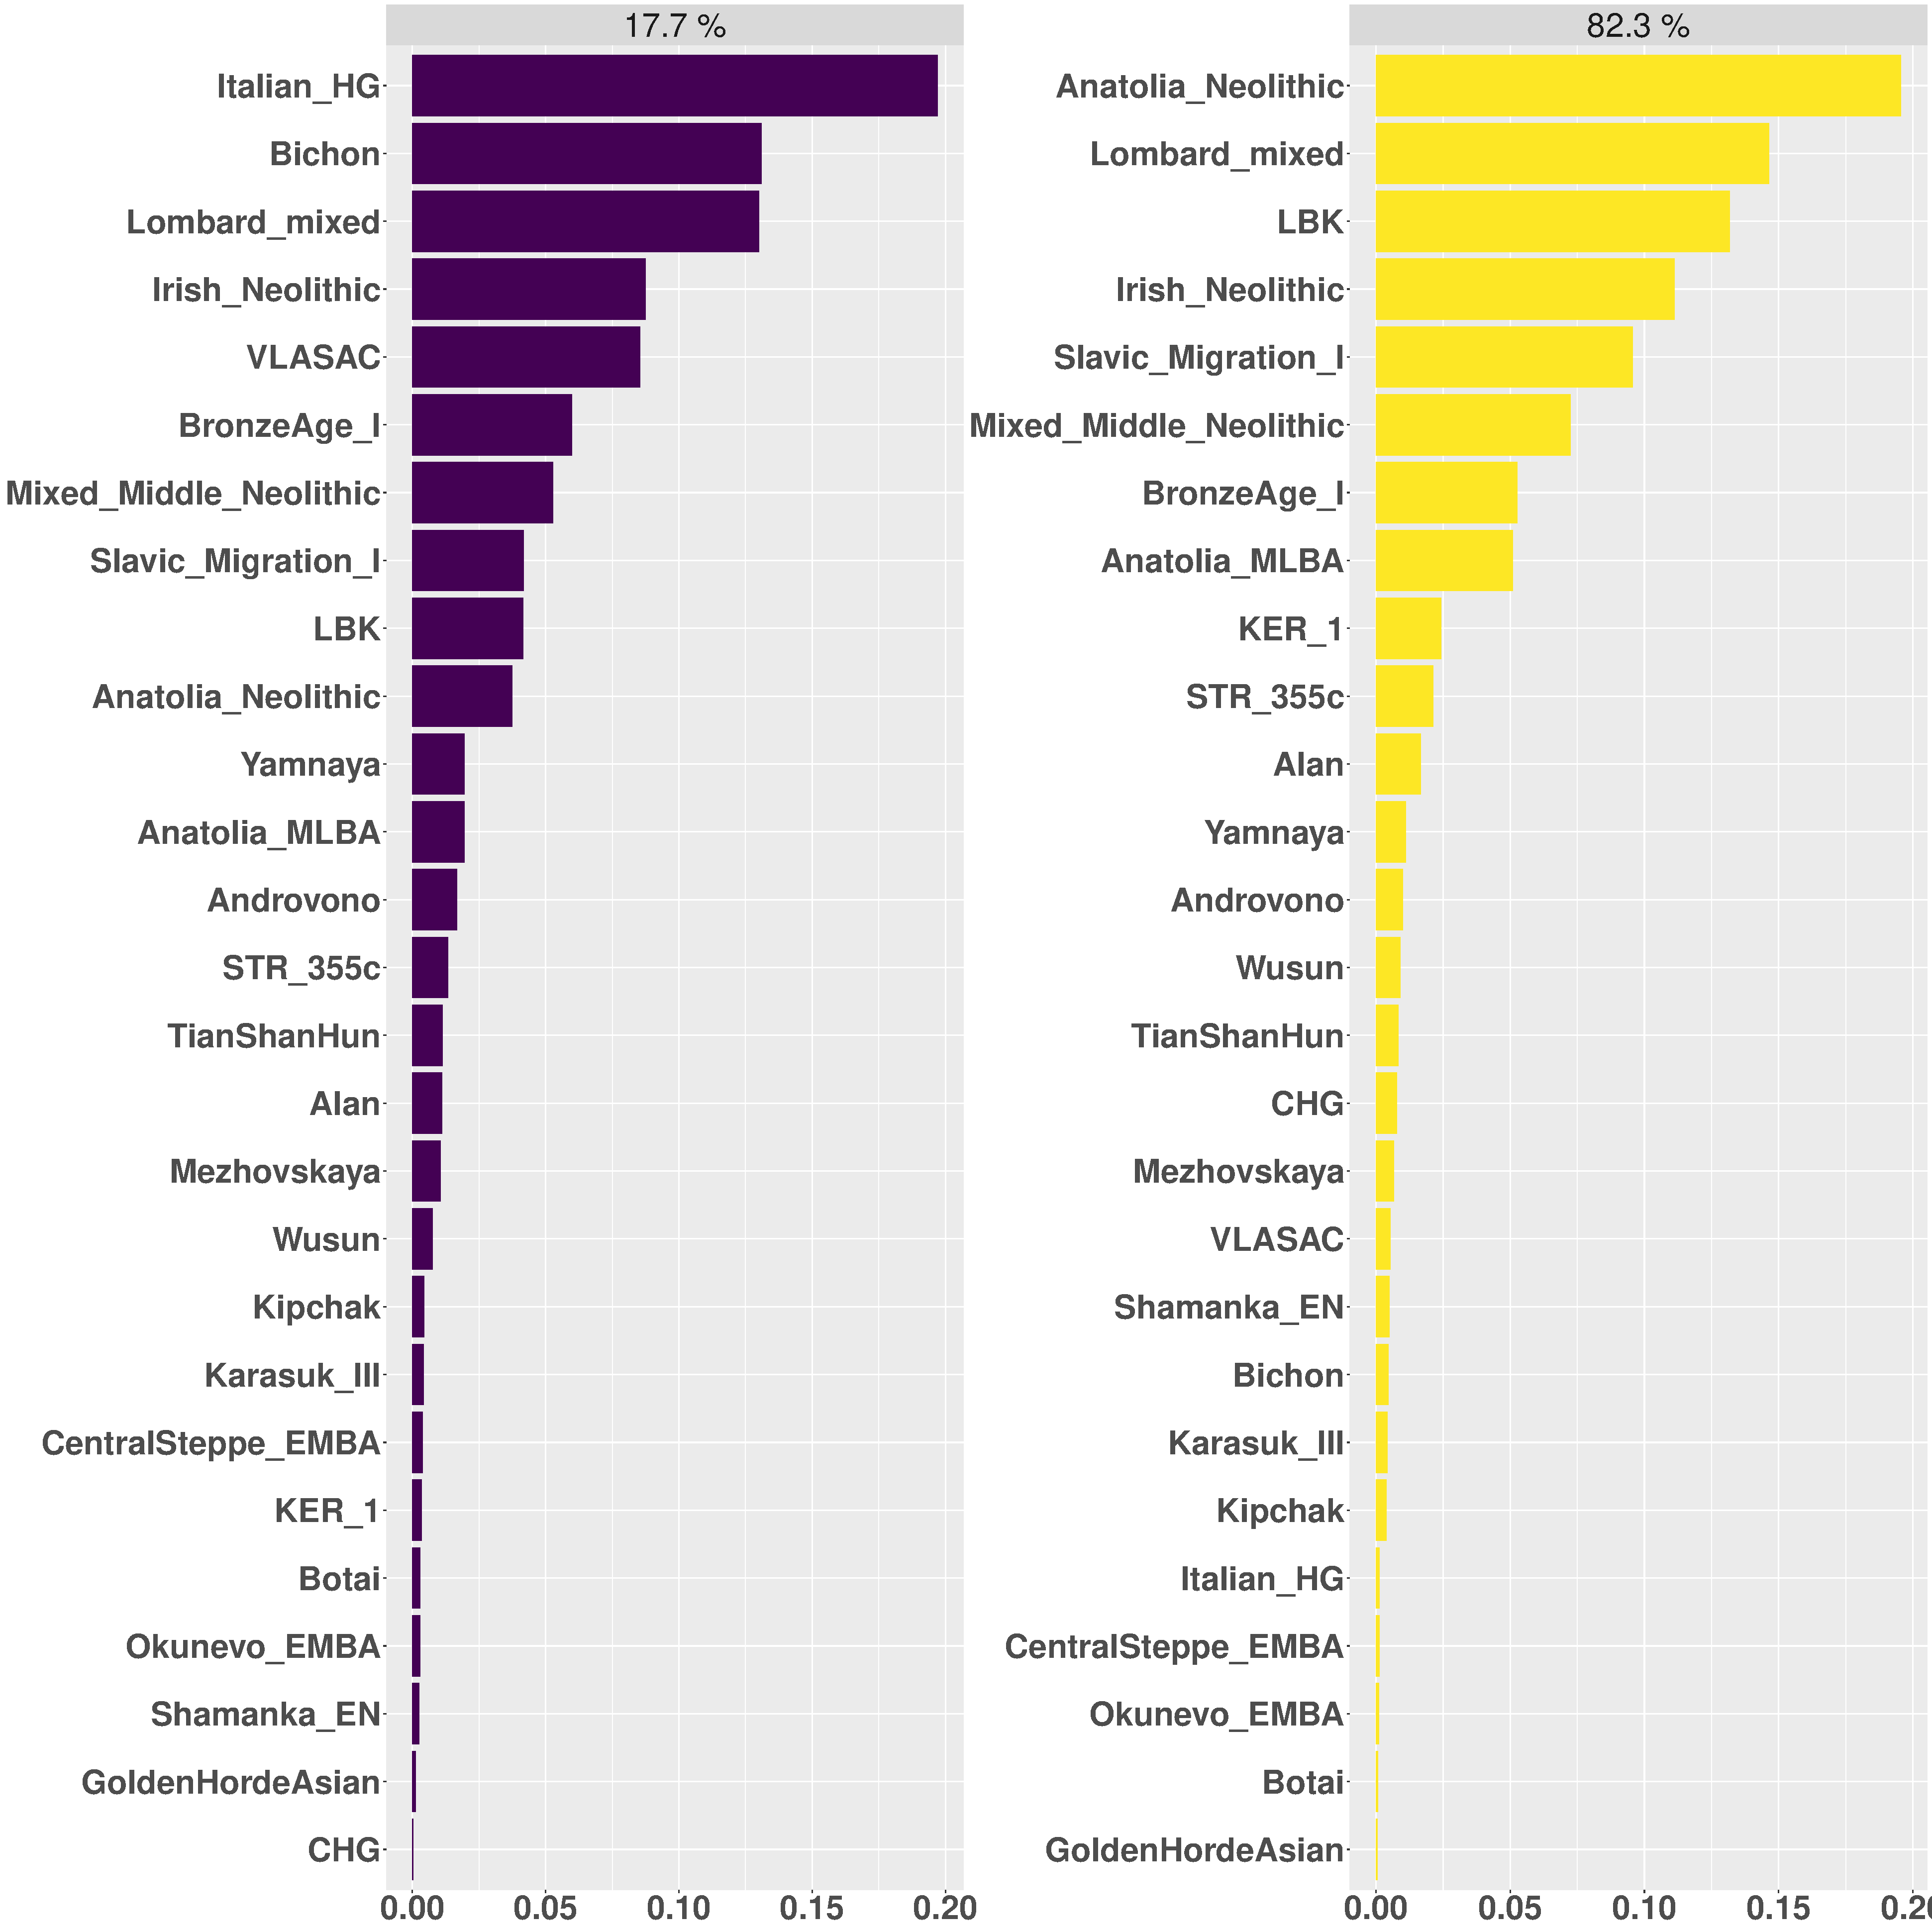
\includegraphics[width=1.0\textwidth]{../images/chapter4/Erg1_MU_matrix.pdf}
    \caption{Copying matrix plot for sources in 2-way admixture event for Erg1. Each panel represents one of the 2 mixing sources. Labels above each panel gives the proportion that mixing source contributed to the Early Middle Age samples. Length of the bars within each panel represent the amount that mixing source copied from a particular population.}
    \label{fig:Erg1_MU_matrix}
\end{figure}



\begin{figure}[htp]
    \centering
    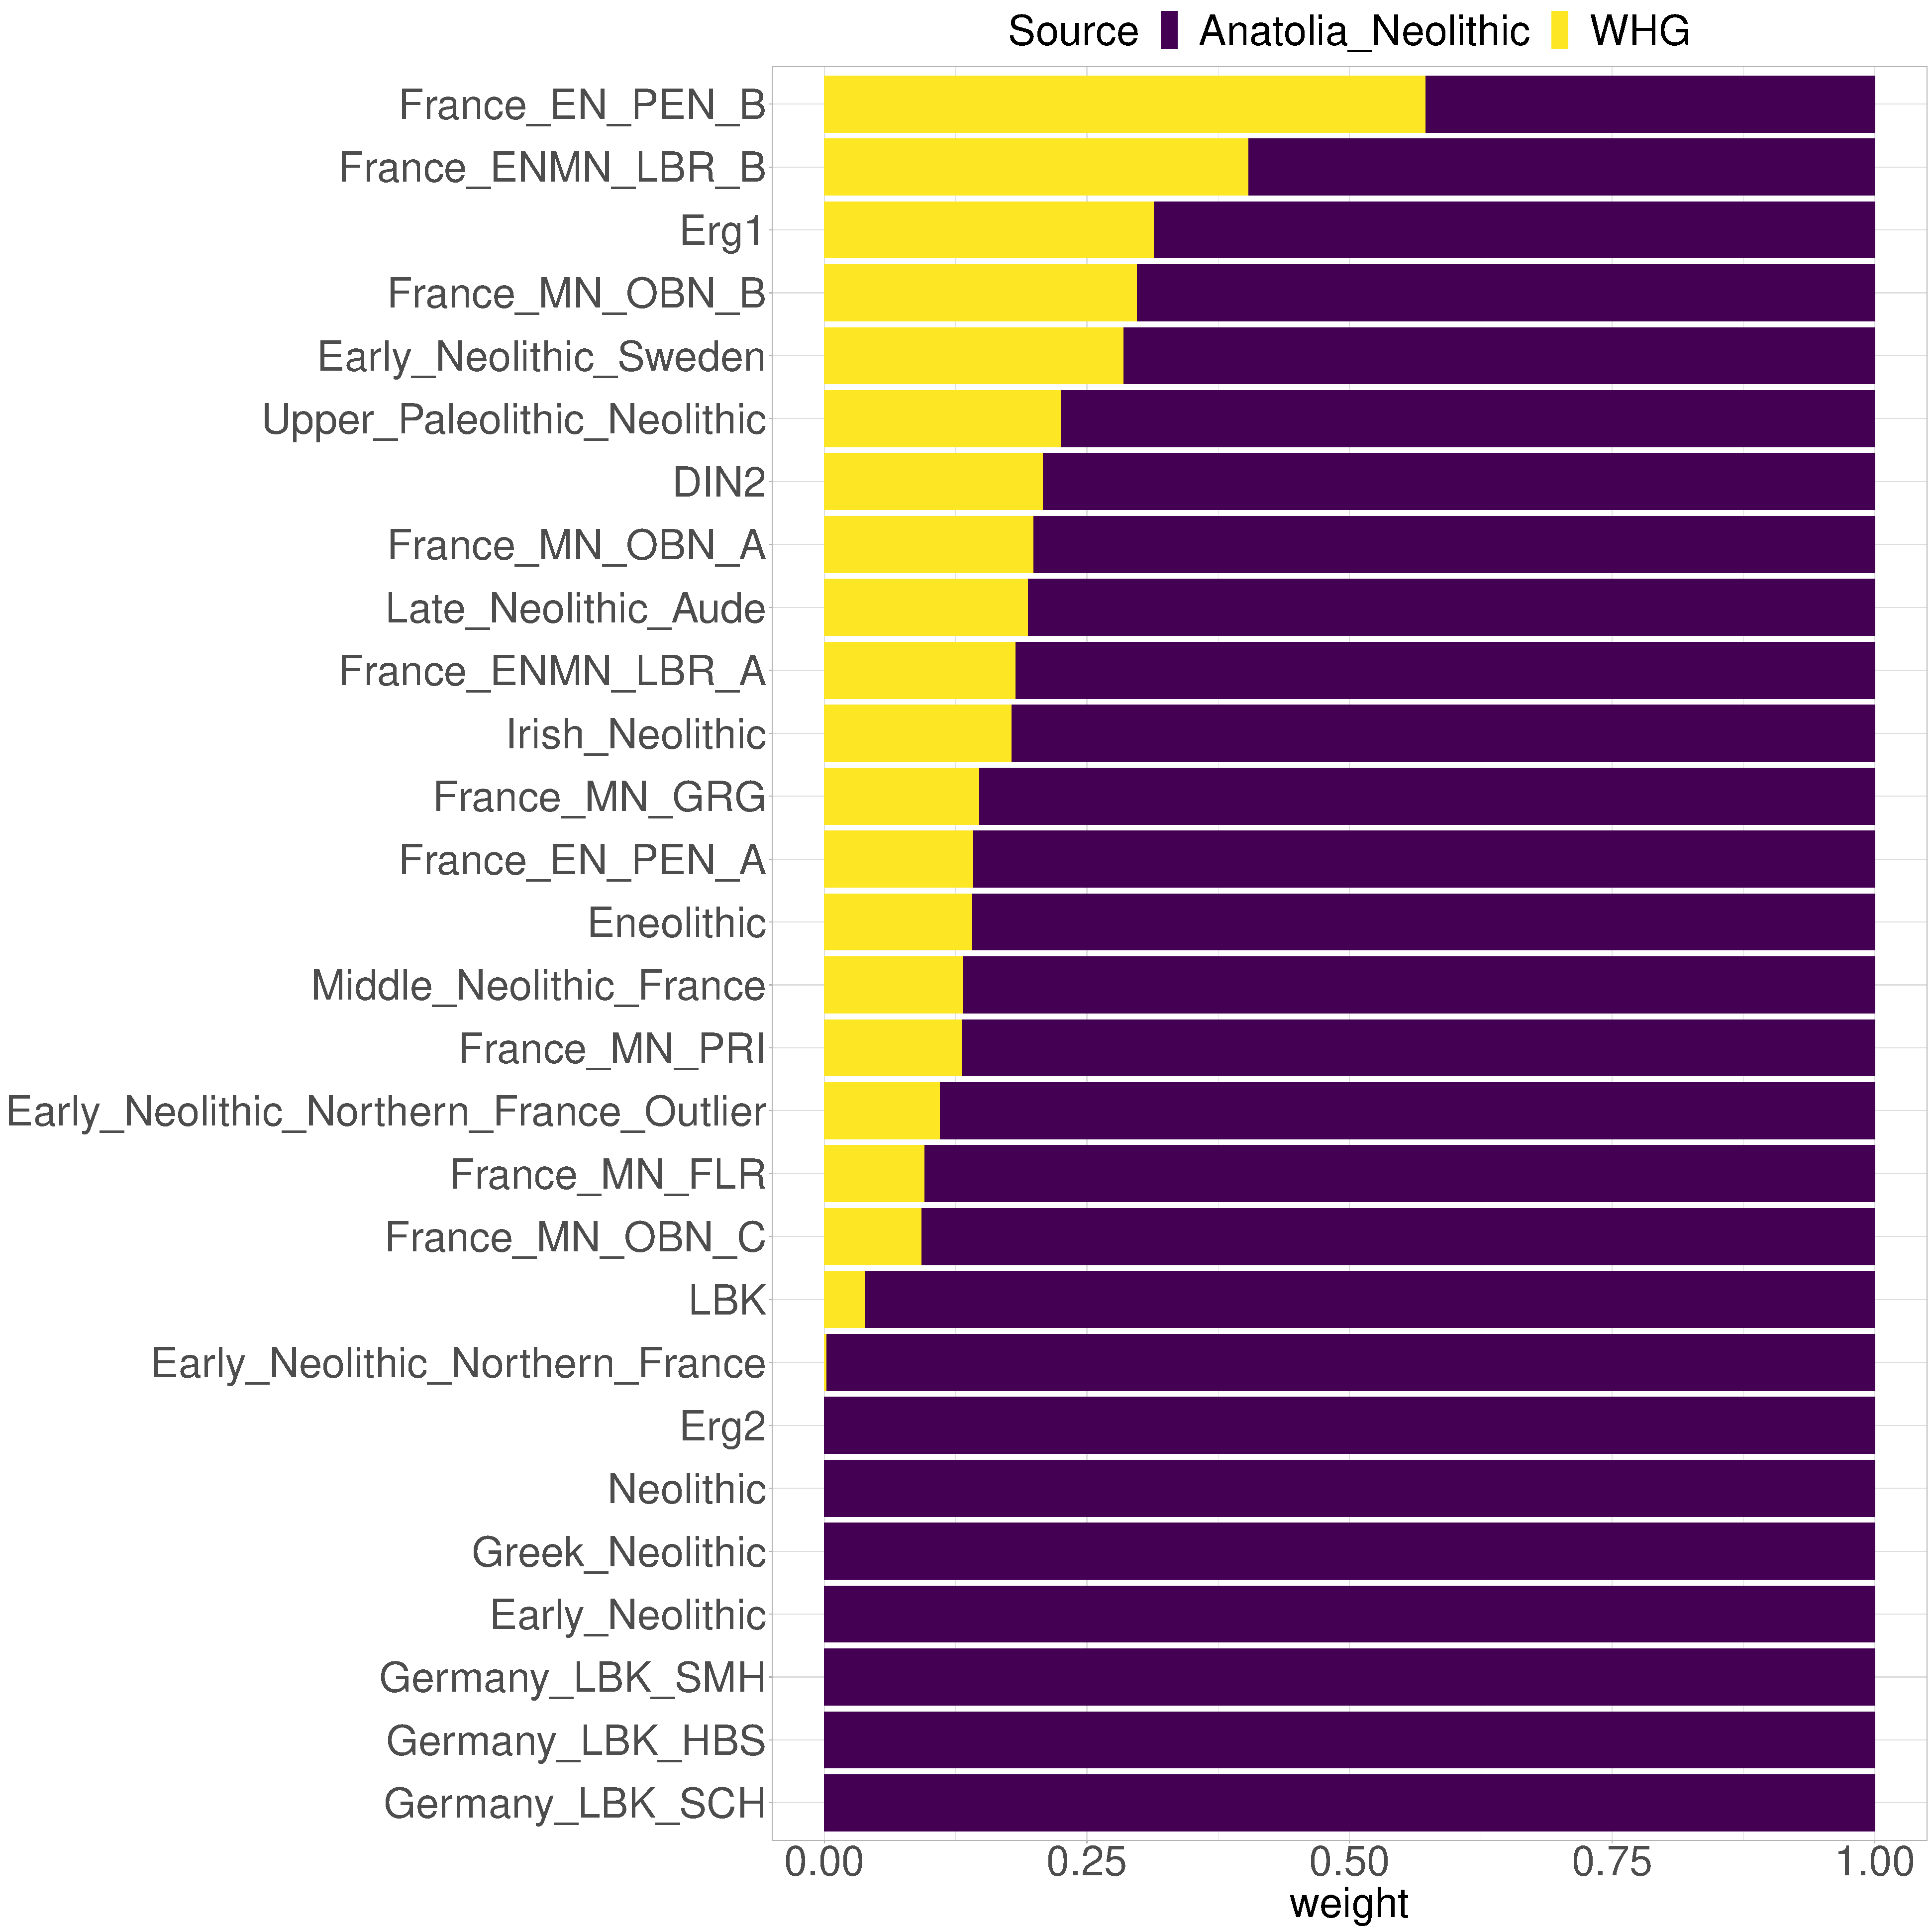
\includegraphics[width=1.0\textwidth]{../images/chapter4/HG_ancestry_Neolithic.pdf}
    \caption{qpAdm ancestry proportion estimates for a selection of European Neolithic individuals. All individuals were modeled as a 2-way mixture between Anatolian Neolithic farmers and Western-Hunter Gatherers (WHG). Outgroups used are \textit{Mota}, \textit{Kostenki14}, \textit{papuan}, \textit{han}, \textit{hannchina}, \textit{mbutipygmy}, \textit{sannamibia}, \textit{yakut}}
    \label{fig:HG_ancestry_Neolithic}
\end{figure}


\begin{figure}[htp]
    \centering
    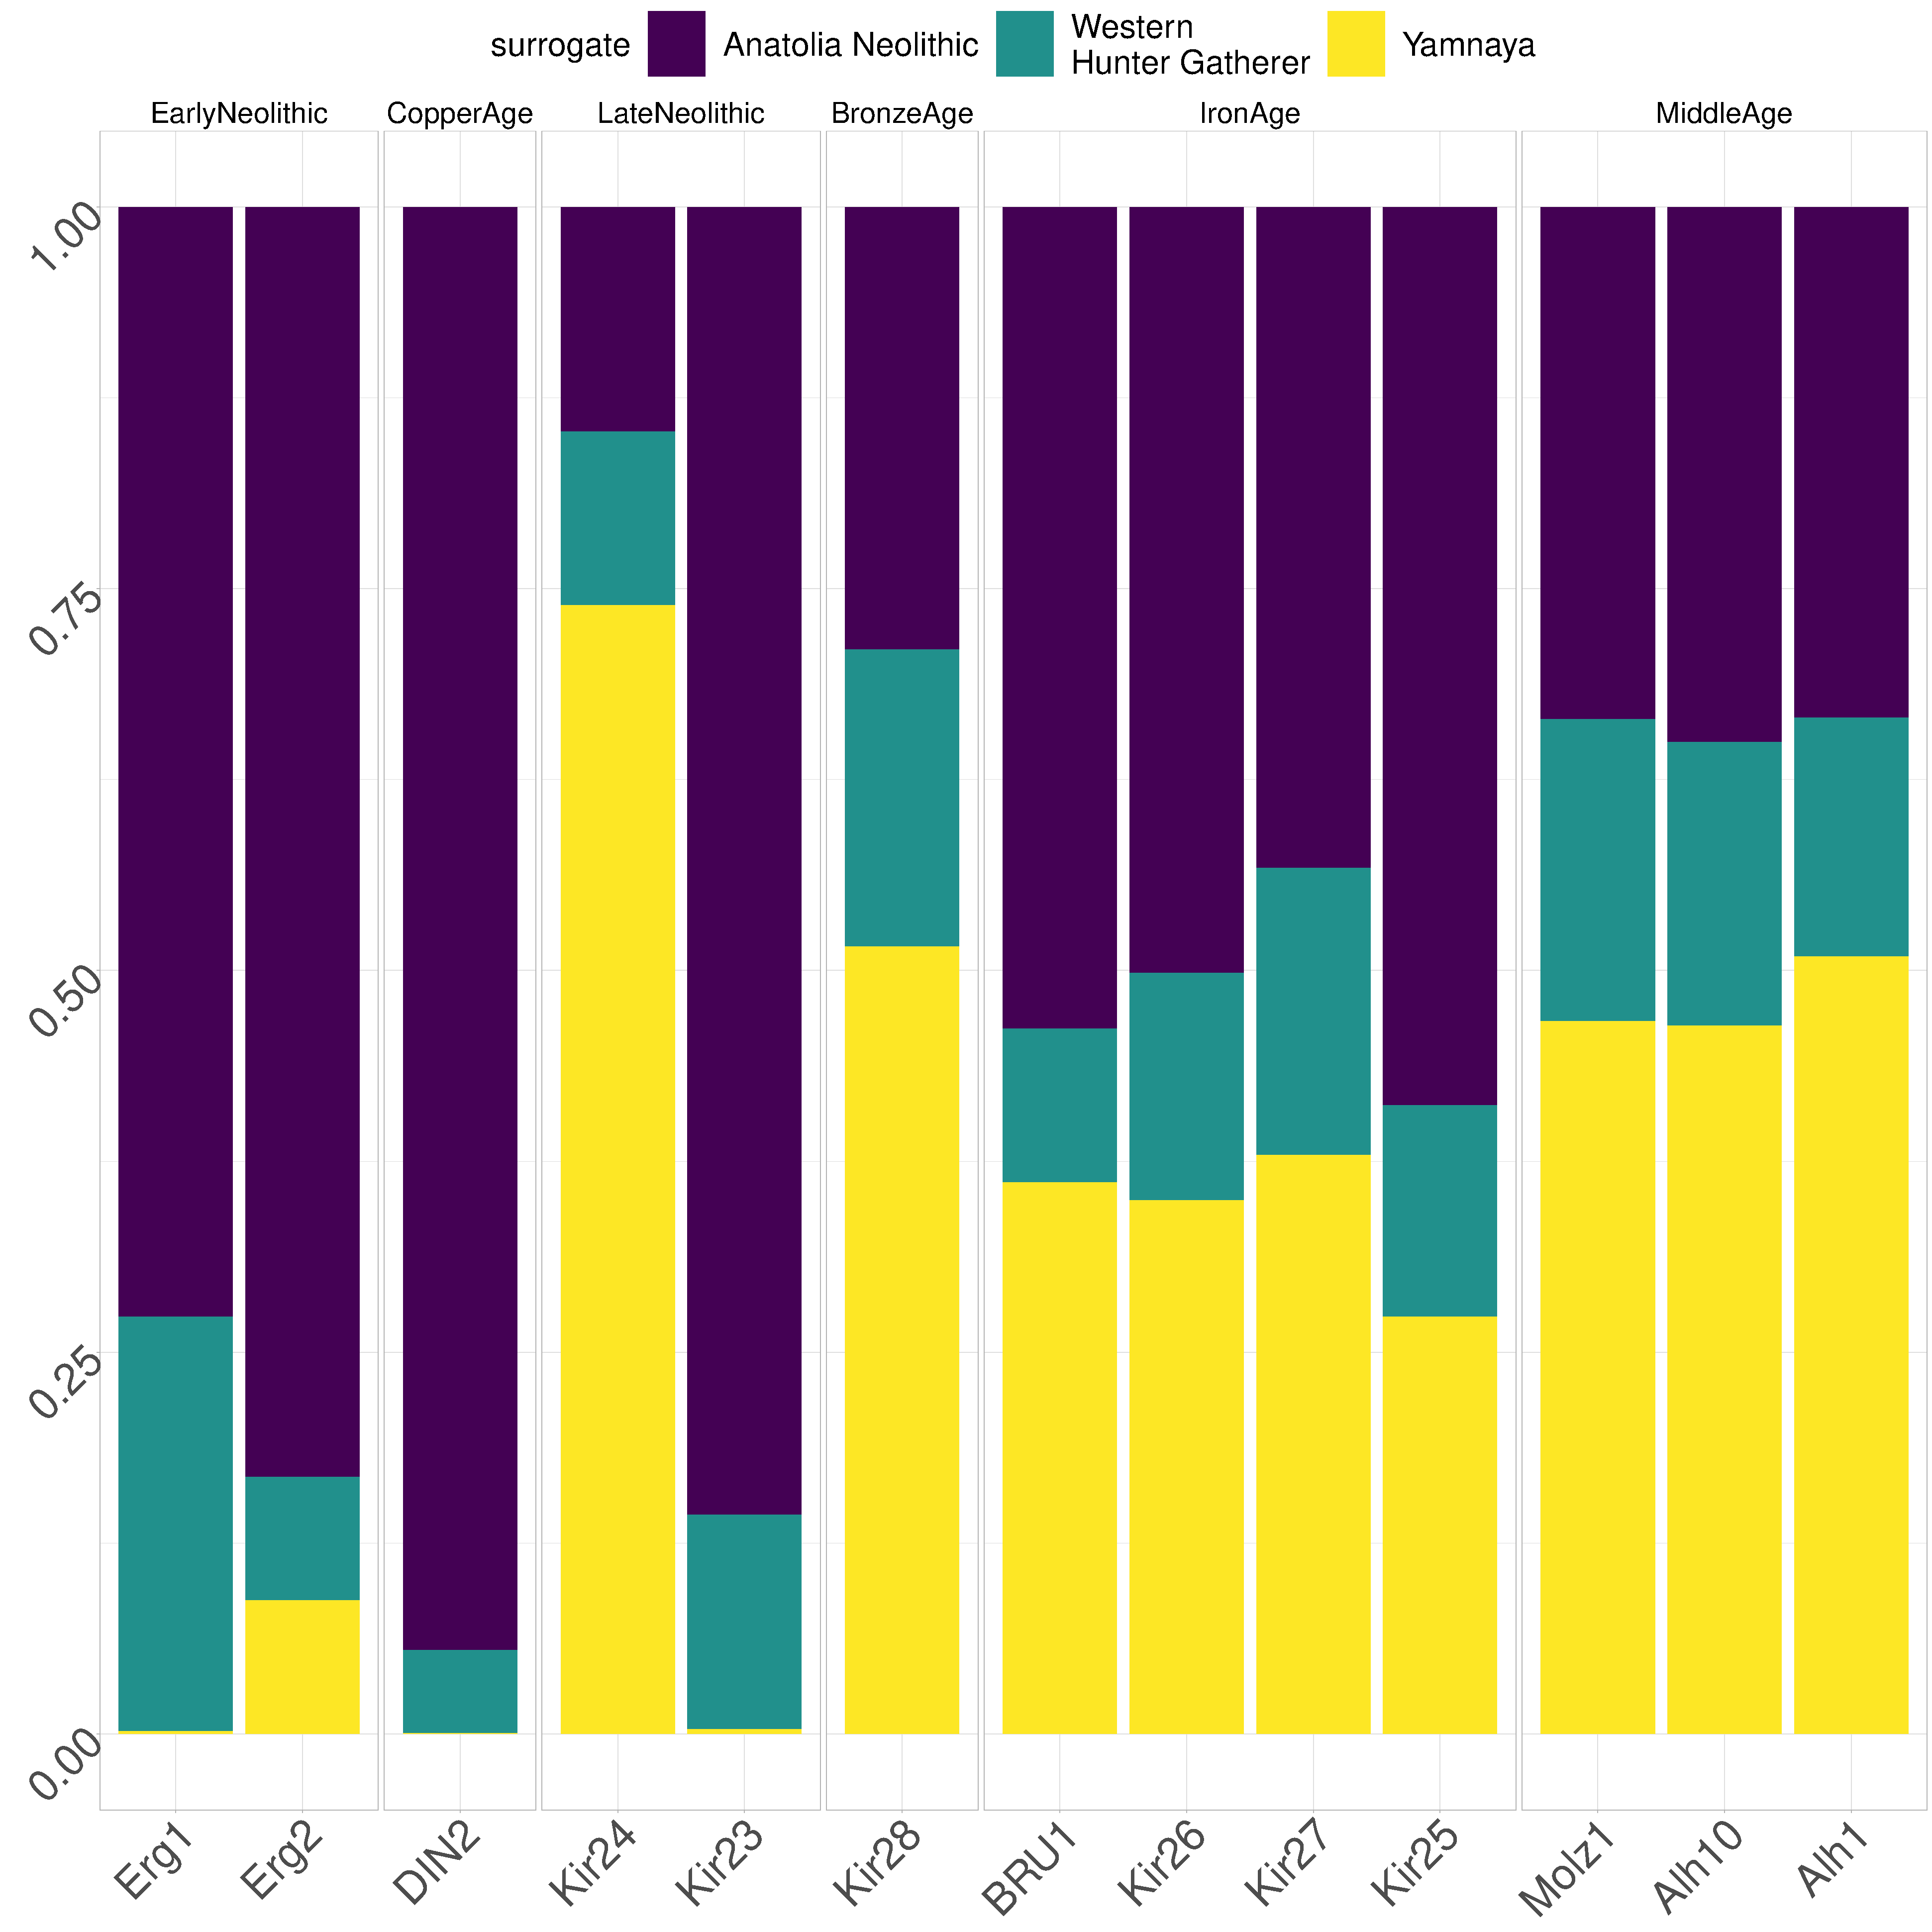
\includegraphics[width=1.0\textwidth]{../images/chapter4/plots3PopBarlot.pdf}
    \caption{SOURCEFIND ancestry proportion estimates for all newly sequenced target samples (vertical columns). Target samples are grouped by archaeological age. Surrogate populations are represented as horizontal rows and also grouped into archaeological culture. Each target was modeled as a mixture of only populations which are dated to being older or contemporaneous as the the target. Numbers within each cell correspond to the ancestry proportion estimate.}
    \label{fig:plots3PopBarlot}
\end{figure}

\subsection{Spatially and temporally close samples in Late Neolithic display highly distinct ancestries}

This dataset included two individuals found in the same stratigraphical layer of Cherry-Tree cave; Kir23 and Kir24 were both dated to the Late Neolithic (approx 4700 BP). Despite their temporal and spatial closeness, they show highly different ancestry profiles (Fig. \ref{fig:plots3PopBarlot}). 

On both the plink PCA and fineSTRUCTURE clustering, Kir24 clusters with individuals from populations present around the Eurasian Steppe during the Bronze-Age, such as those from the Yamnaya and Afanasievo cultures. These are the populations thought to be in part responsible for the spread of Indo-European languages across Europe \cite{Haak2015}.  That the Yamnaya and Afanasievo samples were sampled in Russia suggests that Kir24 may have been a recent migrant from the Eurasian Steppe. This is supported by IBD analysis; of all the ancient samples in the dataset Kir24 shares the most IBD (31.12cM) with the Yamnaya type-specimen and the lowest $TVD$ with 2 other members of the Yamnaya population. This timing (Kir24 is dated to approximately 4700 BP) corresponds to some of the earliest appearance of Yamnaya-like ancestry in central Europe \cite{Racimo8989}. Using qpAdm, Kir24 could be modelled as a mixture of Yamnaya (93\%, se=12) and WHG (6\%, se=8) without any Neolithic ancestry. 

Kir24 was assigned to mtDNA haplogroup T1a1, which has been found in Yamnaya samples from the Middle Volga region and Bulgaria \cite{keyser2009ancient}; the same study found the frequency of T1a1 to be higher in the Yamnaya peoples than in any other ancient or modern population. 

On the other hand, Kir23 is found in a fineSTRUCTURE cluster with Ballynahatty, from Neolithic Ireland (3343-3020 BC), and is positioned on both plink and ChromoPainter PCAs with other late Neolithic samples. It is found in adjacent fineSTRUCTURE groups to samples from Neolithic Spain and Ireland. As is the case with other Neolithic samples of this era, Kir23 has a component of Hunter-Gatherer ancestry; it is known that Middle Neolithic individuals are characterised by admixture with the existing Hunter-Gatherer populations. qpAdm modelling showed that Kir23 could be formed from a mixture of Neolithic Anatolia (96\%, se=14)  and Hunter Gatherer (6.25, se=0.91) without the need for additional Steppe ancestry. 

To test whether the source of Neolithic ancestry in Kir23 was most similar to local populations, I performed $f_{4}$ tests in the form $f_{4}(W=Kir23, X=mbutipygy; Y=test, Z=Erg2)$, which tests whether Kir23 forms a clade with Erg2, a local farmer individual, or $test$, where $test$ was one of several different farmer populations. Erg2 was chosen as the local group because it did not infer any potentially confounding Hunter Gather ancestry. Kir23 always formed a clade with Erg2, suggesting that the source of ancestry into Kir23 was local and that there was a degree of continuity within the region. 


\subsection{`Southern' ancestry to Cherry-Tree Cave during the Iron Age is Italian in origin}

The plink PCA shows that the four Iron Age samples are shifted towards the cluster of Neolithic individuals and away from the samples typical of the European Bronze Age. The same pattern is also seen in the present-day PCA, where the Iron Age samples are shifted substantially towards Spain / Northern Italy relative to the preceding Bronze Age sample which is situated among Northern / Western European populations (Germany, Wales) (Fig. \ref{fig:chunklengths_moderns_ancients_PCA_bav}). 

In fineSTRUCTURE, all four Iron Age individuals were grouped alongside several Lombard samples and a Roman soldier from 300AD. qpAdm modelling showed that the Iron Age samples can be well formed from a mixture of the preceding Bavarian Bronze age sample and those from either Renaissance Italy, Imperial Rome, Imperial Rome Late Antiquity or `Roman Solider' from Veeramah et al (2018), with all other possible sources included with Bronze Age giving a poorly fitting models (Table \ref{tab:IronAge_qpAdm}). This suggests a model of admixture from populations best represented by those from post Iron-Age Italy. SOURCEFIND using all ancients as surrogates, inferred 26\% of the IA samples' ancestry was most closely related to the ``Rennaisance'' Italy population from 1500CE, with no such inferred ancestry in the temporally flanking Bronze and Middle Age samples.

\begin{table}
\centering
\begin{tabular}[t]{llrrr}
\toprule
Target & Left & Weight & SE & Z\\
\midrule
Bavaria Iron & Bavaria Bronze & 1.458 & 0.732 & 1.992\\
Bavaria Iron & HallstattBylany & -0.458 & 0.732 & -0.625\\
\addlinespace
Bavaria Iron & Bavaria Bronze & 0.956 & 0.426 & 2.245\\
Bavaria Iron & Renaissance & 0.044 & 0.426 & 0.103\\
\addlinespace
Bavaria Iron & Bavaria Bronze & 0.986 & 0.202 & 4.871\\
Bavaria Iron & Imperial Rome Late Antiquity & 0.014 & 0.202 & 0.070\\
\addlinespace
Bavaria Iron & Bavaria Bronze & 0.990 & 0.173 & 5.738\\
Bavaria Iron & Imperial Rome & 0.010 & 0.173 & 0.056\\
\addlinespace
Bavaria Iron & Bavaria Bronze & 0.981 & 0.280 & 3.505\\
Bavaria Iron & Roman Solider & 0.019 & 0.280 & 0.069\\
\bottomrule
\end{tabular}
\caption{Selected qpAdm results for estimating proportions of ancestry in the four Bavarian Iron Age samples. Each two rows is one test, with left populations as Bavaria Bronze and other. `Weight' gives proportion of ancestry, `SE' jackknifed standard error of Weight. Note negative Weight for model involving  HallstattBylany, showing that the model does not fit well}
\label{tab:IronAge_qpAdm}
\end{table}


MOSAIC inferred the Iron Age samples could be formed of a mixture of $\approx$ 18\% ancestry from a source closest to an Alamannic-Frankish sample (510 – 530 AD) and $\approx$82\% ancestry from a source closest to Anatolian Neolithic / LBK samples, with admixture dated to 9.2 generations ago (bootstrapped 95\% CI: 7.86-11.31). $F_{st}$, estimated by MOSAIC, between the two mixing sources was 0.016, approximately equivalent between present-day Germans and Palestinians \cite{nelis2009genetic}.  


Based on SOURCEFIND and qpAdm modelling with selected ancient and present-day East Asian samples, unlike Gamba et al (2014) \cite{Gamba2014}, I found no evidence of East-Asian or East-Asian-like admixture (Fig. \ref{fig:chapter4resultsSFheatmapolder}).


\subsection{Present-day genomes unpick genetic differences between early Germanic and Slavic populations}

Lastly, my dataset included three samples (1 newly sequenced) from the Middle Age period. The two genomes from Altheim, Germany, date to around 500AD and were found in a Roman context. The single individual from Molzbichl, Austria, dates to around 300 years later, and has been assigned to a `Slavic' cultural context. It is currently unknown whether, in addition to cultural and linguistic differences, genetic differentiation exists between the `Germanic’ peoples represented by the two Altheim samples, and the `Slavic’ peoples represented by the Molzbichl sample.

The three Middle Age samples appear to share common ancestry based on the plink PCA and are located next to other spatially and temporally close samples from the Middle Ages. Similarly, they have almost indistinguishable SOURCEFIND ancestry proportions (Fig \ref{fig:plots3PopBarlot}).

$f_{4}$ in the form $f_{4}(mbutipygymy, Bavaria\_Iron; Bavaria\_Slav, Bavaria\_Germanic)$ returned a non-significant result, consistent with `Germanic' and `Slavic' populations splitting post Iron Age. However this non-significant result could be caused by low sample sizes in the Middle Age populations or a lack of power in allele-frequency based methods.

However, the two Germanic samples fall into a fineSTRUCTURE cluster with a set of contemporaneous samples from Northern Europe, including 10-11\textsuperscript{th} century Vikings from Estonia, Sweden and Iceland, whereas Molz1 clusters with other individuals known to be from Early Slavic populations. Interestingly, the Slavic cluster also containing a sample DA29, also know as `GoldenHordeEuro'. This sample is from Karasuyr, Kazakhstan, and has dated to 1200-1400 CE. The Golden Horde was a Mongol khanate established in the 13th Century CE. Given this sample shows clear evidence of European ancestry and clusters alongside individuals from Early Middle Age Europe, it has been proposed that this individual was captured in Europe during the Mongol raids of the 13th Century, when they assaulted the Kievan Rus' federation \cite{de2018137}. That `GoldenHordeEuro' clusters with Molz1 suggests the location of capture in Europe may have been from Austria where Molz1 was found.

On a haplotype-based PCA with modern samples, Molz1 clusters with present-day Slavic speaking populations such as Poland, Ukraine and Belarus, while the two Germanic samples cluster with present-day individuals from Germanic-speaking countries in Western Europe, such as Scotland, Germany and Wales (Fig. \ref{fig:chunklengths_moderns_ancients_PCA_bav}). Plotting differential haplotype sharing between the Slavic and Germanic sample makes this pattern clear (Fig \ref{fig:germanic_slavic_HB_sharing}). There is a clear division down the centre of Europe, dividing it into East and West that shows the structure in present-day Europeans has existed since at least the Early Middle Ages. 

In SOURCEFIND, the two samples from Altheim derived a large proportion of their ancestry to modern day Germans (81.8\%, se=12.8), whereas the Molzbichl sample derived a large proportion of its ancestry from modern day Polish (77.85\%, se=20.3) and Croatians (11.7\%, se=9.1). 

\begin{figure}[htp]
    \centering
    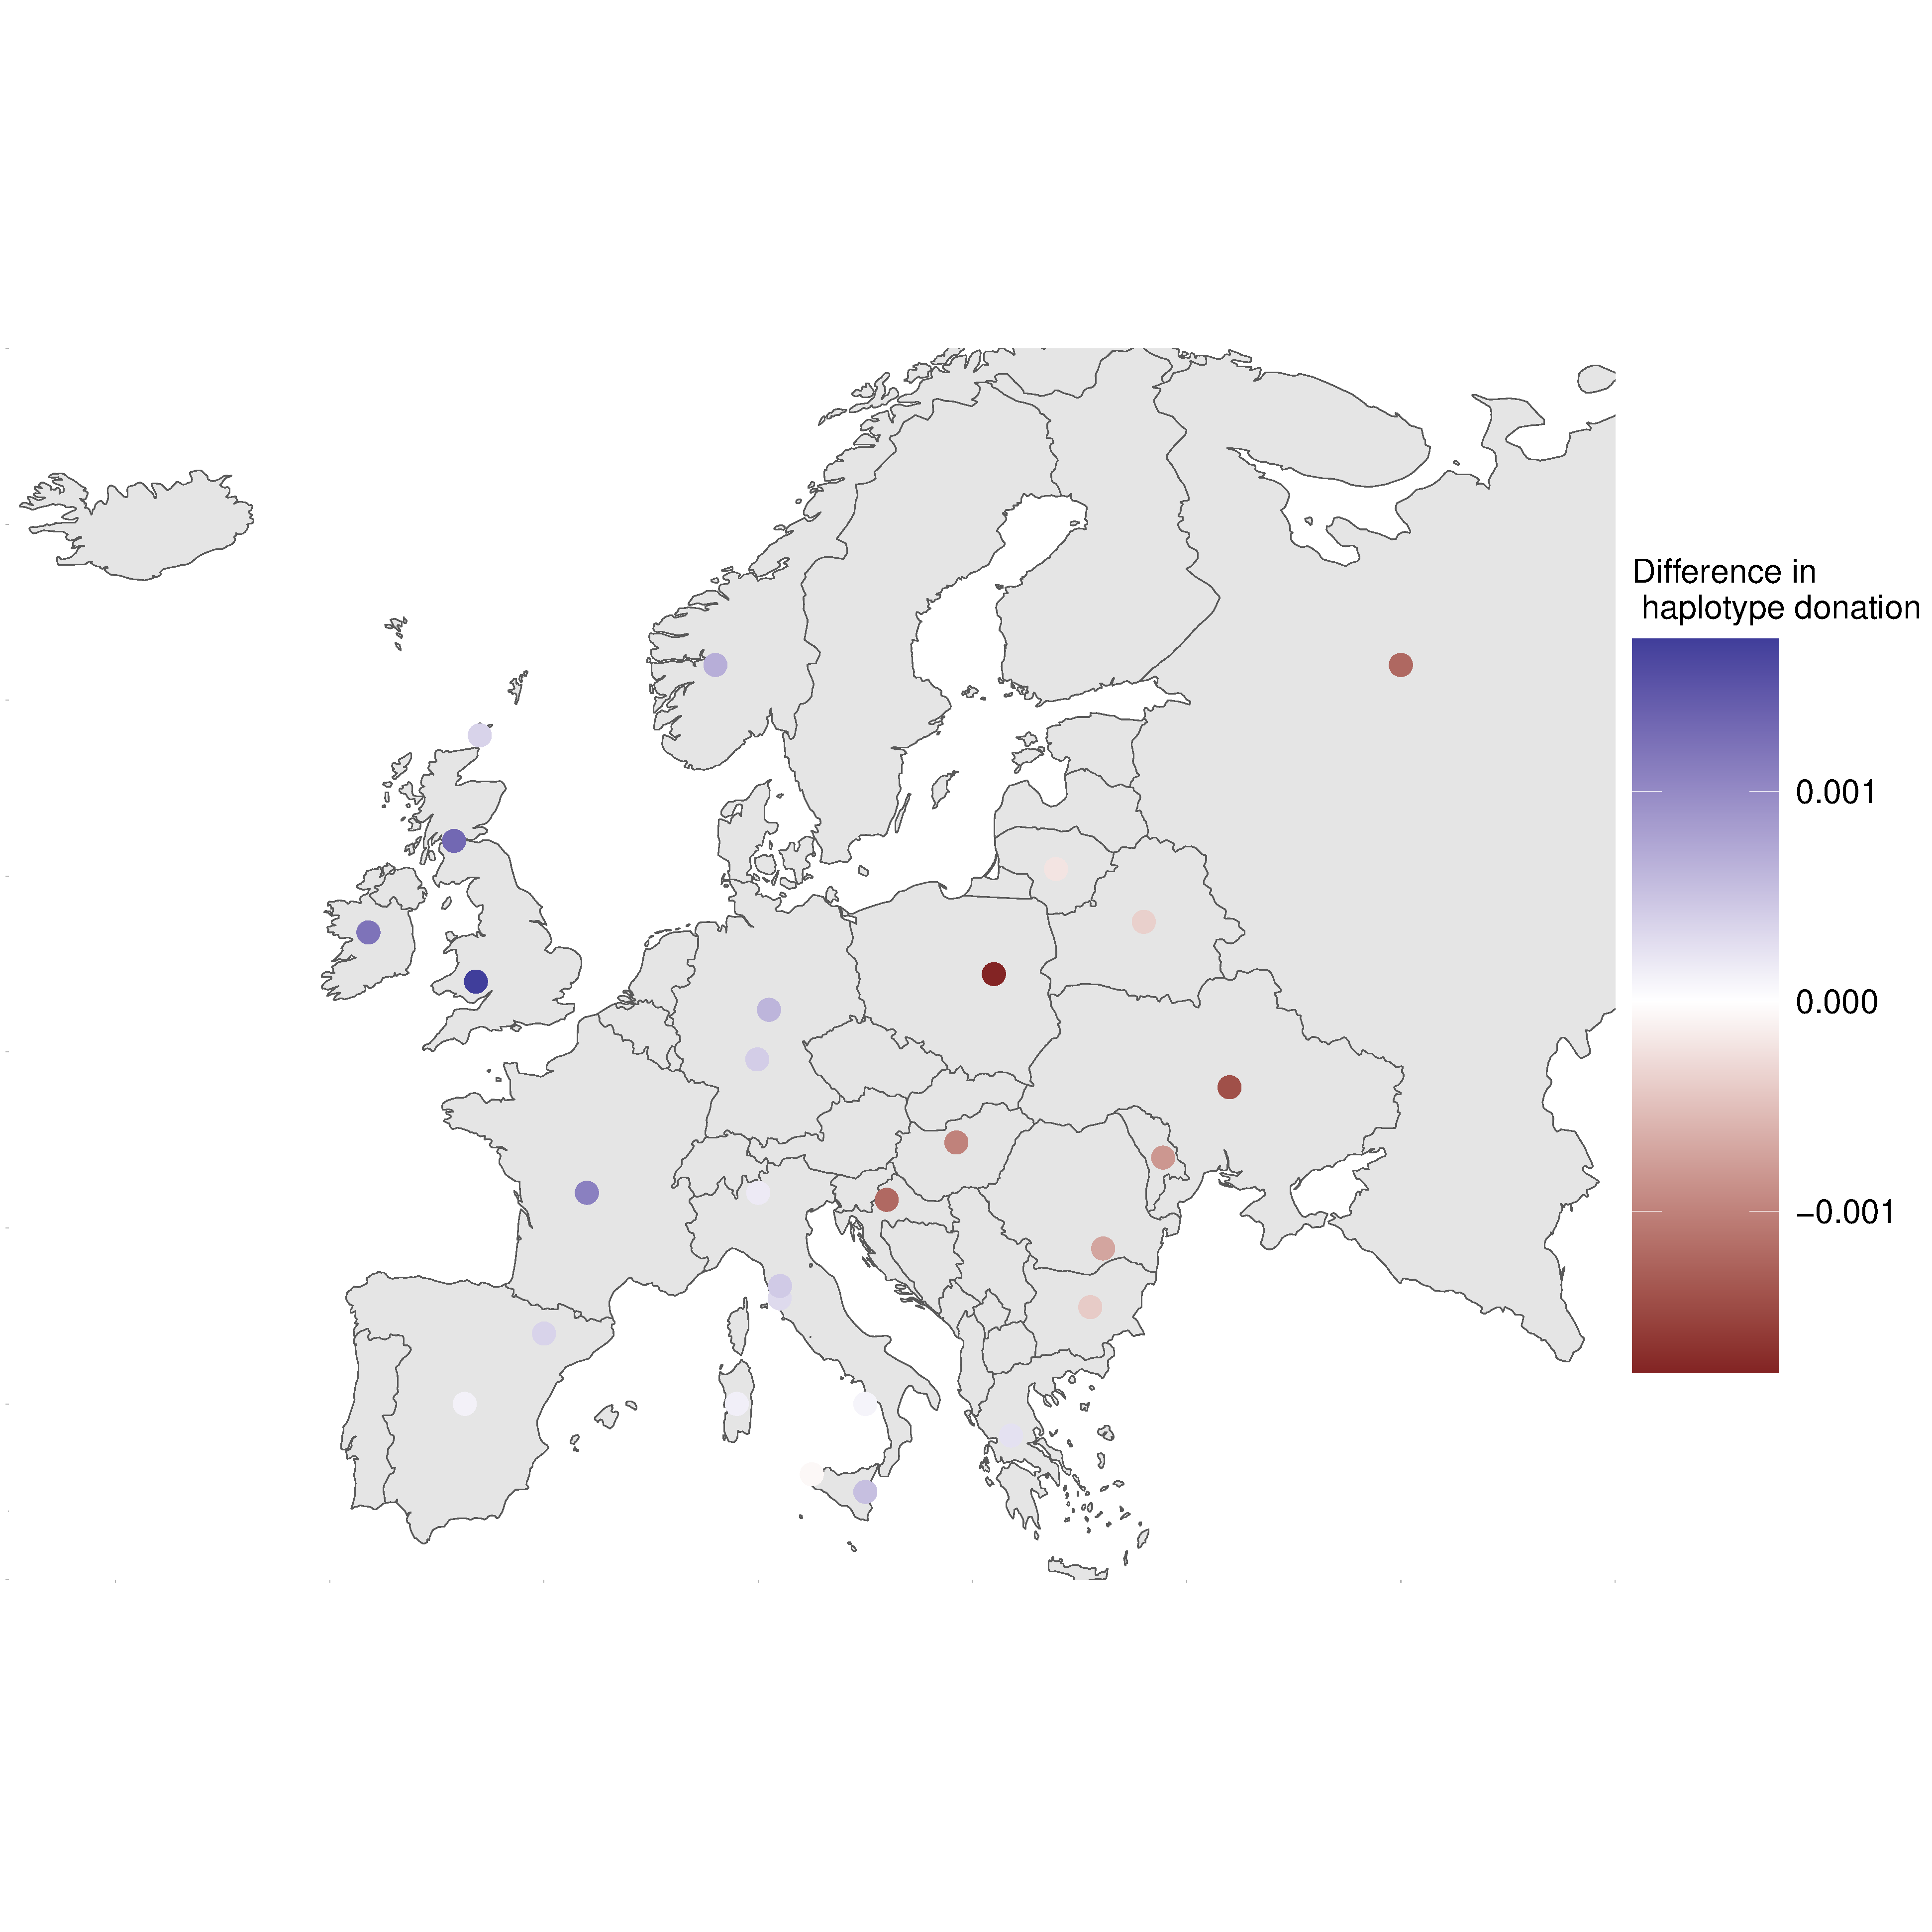
\includegraphics[width=1.0\textwidth]{../images/chapter4/germanic_slavic_HB_sharing.pdf}
    \caption{Differential haplotype-donation between Germanic and Slavic samples. Each coloured point is one present-day population. Points are coloured based on whether they donate relatively more to Germanic (blue) or Slavic (red) ancient samples.}
    \label{fig:germanic_slavic_HB_sharing}
\end{figure}

\subsection{Summary of Results and Discussion}

Drawing back to the questions asked at the beginning.

Whilst the two samples from the Early and Middle Neolithic, Erg1 and DIN2, showed some signs of being from at least closely related source populations, they also displayed variation suggestive of different population histories. Consistent with the hypothesis that DIN2 may have migrated along the Danubian route, it shares the lowest $TVD$ and is found in a fineSTRUCTURE cluster with other samples from the Hungarian Plane. Most importantly, Erg1 and DIN2 two samples also showed differences in the degree of Hunter-Gatherer ancestry; whilst DIN2 showed no evidence of admixture, Erg1 likely had a recent Hunter-Gatherer ancestor.

I found evidence of population discontinuity in Cherry-Tree Cave from the Late Neolithic through to Iron Age. I identified a incoming signal of `southern' ancestry during the Iron Age, which was not present in the single sample from the preceding Bronze Age. The most plausible source of this ancestry is from Italy, with the best source in the dataset being the cluster of Renaissance samples from Antonio et al (2019) \cite{antonio2019ancient}, date to between 282 - 354 AD. This, combined with evidence the Iron Age samples cluster with present-day individuals from north Italy and historical evidence of Lombard migrations to Southern Germany \cite{wegewitz1972}, suggests they may be the admixing source. Whilst collaborators proposed that the source may be related to the local Hallstatt culture, qpAdm modelling rejected this scenario (Table \ref{tab:IronAge_qpAdm}). Wherever the source originated from, this admixture event provides strong evidence against continuity in Cherry-Tree Cave. 

Lastly, I used present-day genomes of individuals from across Europe to show that there are clear genetic differences between the Middle Age Germanic and Slavic samples, with the Germanic samples showing a strong affinity to western European countries and the Slavic samples showing a strong affinity to eastern European samples (Fig. \ref{fig:germanic_slavic_HB_sharing}). However, in the context of ancient samples, all three Middle Age samples clustered with local samples from the Bronze Age rather than the Iron Age (Fig. \ref{fig:plink_PCA}). 

This dataset revealed that temporally and spatially close samples may have very distinct genetic ancestry profiles, with Early Bronze Age samples Kir24 and Kir23 showing high levels of Steppe-related and Neolithic ancestry respectively. In particular, Kir24 seemed to be very recently related to the Yamnaya type-specimen sample, sharing 31cM of IBD with it. The arrival of Yamnaya-like ancestry from this early (2762BC) represents one of the earliest known appearances in the literature. 

Future studies in this region should focus on obtaining a higher density of samples, in particular from the Bronze and Iron Ages; the low number of samples from these time periods mean any results should be interpreted with caution. More samples would show whether the introduction of `southern' like ancestry in the Iron Age was a widespread phenomena, or restricted to a smaller geographic region in Southern Germany. Similarly, a wider sampling of Iron Age groups from Germany, Italy and Switzerland may allow for a more accurate identification of this source.

Whilst the utility of using present-day genomes was outlined through the comparison of the Slavic and Germanic samples, the analysis would have been significantly improved with higher resolution data from Germany. The data I have, described in Appendix section \ref{section:MSPOBIHellBus}, only had country-level details. Data which had labels from different sub-regions in Germany, similar to the POBI dataset, would have allowed for a finer-scale investigation into the current east-west genetic divide in present-day Germany.    

